%%%%%%%%%%%%%%%%%%%%%%%%%%%%%%%%%%%%%%%%%%%%%%%%%%%%%%%%%%%%%%%%%%%%%%%%%%%%%%%%%%%%%%%%%%%%%%%%%%%%%%%%%%%%%%%%%%%%%%%%%%%%%%%%%%%%%%%%%%%%%%%%%%%%%%%%%%%%%%%%%%%%%%%
%%%%%%%%%%%%%%%%%%%%%%%%%%%%%%%%%%%%%%%%%%%%%%%%%%%%%%%%%%%%%%%%%%%%%%%%%%%%%%%%%%%%%%%%%%%%%%%%%%%%%%%%%%%%%%%%%%%%%%%%%%%%%%%%%%%%%%%%%%%%%%%%%%%%%%%%%%%%%%%%%%%%%%%
\FloatBarrier
\chapter{Optimisation of the search sensitivity}
\label{sec:Optimisation}
Finally, having all background estimation methods in place, an optimisation procedure is conducted in order to increase the search sensitivity with respect to different signal models as introduced in Section~\ref{sec:SignalSamples}.
The optimisation is done in the most sensitive variables, \pt and \ias (see Section~\ref{sec:Ias} for a definition and explanation of the Asymmetric Smirnov discriminator \ias).
A potential additional discriminating variable is the number of missing outer hits \nlostouter in the tracker system. 
This variable is, however, not considered in this analysis because studies show that the discriminating potential is limited (see Appendix~\ref{app:OptimisationNLostOuter}).\\

SUSY models with different chargino lifetimes and masses are characterised by different \pt and \ias distributions as well as different theoretical cross sections.
Therefore, the usual search optimisation strategy that maximises $N_S/\Delta B$ ($N_S$ = number of signal events of model $S$, $\Delta B$ = background uncertainty) implies a potential fine-tuning on the specific SUSY cross sections.
In order to keep the search as general as possible, a cross section independent optimisation is performed.
This is achieved by a minimisation of the cross section for which a 5$\sigma$-discovery of the corresponding signal model is possible, \ie finding the optimal selection cuts for \pt and \ias for which the lowest possible cross section, $\sigma_{\text{min}}$, can be discovered
\begin{align}
\label{eq:optimisation}
%\frac{\sigma_{\text{min}}\cdot \mathcal{L}}{\Delta B} = \frac{\sigma_{\text{min}}\cdot \mathcal{L}}{\sqrt{ \left(\Delta B_{\text{stat}}\right)^2 + \left(\Delta B_{\text{sys}}\right)^2}} \geq 5.
\frac{\alpha_{\text{min}} \cdot N_S(\text{mass},\ctau,\pt^{\text{cut}}, \ias^{\text{cut}})}{\Delta B (\pt^{\text{cut}}, \ias^{\text{cut}})} = 5. && \text{with   } \alpha_{\text{min}} = \frac{\sigma_{\text{min}}}{\sigma_{S}}.
\end{align}
The number of expected events $N_S$ of the signal model $S$ depends on the \pt and \ias selection cut as well as the mass and the lifetime of the chargino.
The uncertainty on the background $\Delta B$ is dependent on the \pt and \ias cut, and takes into account the full systematic uncertainty as well as the statistical uncertainty on the background prediction which is the 68\% one sided upper limit of a Poisson distribution with $\mu = N_B$ estimated with the Neyman construction~\cite{bib:Neyman_1937,bib:PDG_2014}.
The systematic uncertainty on the background prediction includes systematic uncertainties as described in Section~\ref{sec:SysUncertaintiesBkg}, and statistical uncertainties arising from limited statistical precision of the control regions and simulated samples used in the background estimation.
The factor $\alpha_{\text{min}}$  that is minimised is the ratio of the minimum cross section $\sigma_{\text{min}}$ divided by the nominal cross section $\sigma_{S}$ of the signal model S.\\

As this analysis focuses on short tracks, rather low lifetimes are considered in the optimisation procedure: $\ctau=1\cm,\,10\cm,\,50\cm$.
These lifetimes are further suitable as they lie at the edge of the sensitivity of the search for disappearing tracks~\cite{bib:CMS:DT_8TeV}.
To cover the full mass space, the optimisation is done for masses between 100\gev and 500\gev.
The corresponding results are shown in Table~\ref{tab:optimisation}.
\renewcommand{\arraystretch}{1.5}
\begin{table}[!h]
\centering
\caption{Optimal \pt and \ias selection cuts and the corresponding minimum cross section $\sigma_{\text{min}}$ that can be discovered with 5$\sigma$ significance for different signal models.
         For some signal samples, an optimisation result is not available due to the limited size of these samples.}
\label{tab:optimisation}
\makebox[0.99\textwidth]{
\begin{tabular}{c |c| c| c| c}
\multicolumn{5}{c}{} \\
\toprule
Mass [\gev] & Lifetime [\cm] & Optimal \pt cut & Optimal \ias cut & $\sigma_{\text{min}}$ \\
\midrule
100&                     1&                       30&                      0.05&                    61.596\\
200&                     1&                       20&                      0.05&                    43.414\\
300&                     1&                       n/a &                    n/a &                    n/a \\  
400&                     1&                       n/a &                    n/a &                    n/a \\  
500&                     1&                       n/a &                    n/a &                    n/a \\  
\midrule
100&                     10&                      30&                      0.05&                    1.531\\ 
200&                     10&                      30&                      0.30&                    0.561\\ 
300&                     10&                      30&                      0.30&                    0.354\\ 
400&                     10&                      30&                      0.30&                    0.238\\ 
500&                     10&                      50&                      0.30&                    0.201\\ 
\midrule
100&                     50&                      50&                      0.30&                    0.435\\ 
200&                     50&                      50&                      0.30&                    0.110\\ 
300&                     50&                      50&                      0.30&                    0.063\\ 
400&                     50&                      50&                      0.30&                    0.045\\ 
500&                     50&                      50&                      0.30&                    0.037\\ 
\bottomrule
\multicolumn{5}{c}{} \\
\end{tabular}}
\end{table}

It can be seen that the optimal selection is highly dependent on the signal models.
The best sensitivity for low masses ($\leq 200\gev$) is mainly achieved by soft selection cuts in \pt between $20-30\gev$, while models with higher chargino masses require tighter \pt selections of around 50\gev.
The optimal \ias selection is mostly dependent on the mass of the chargino.
For low masses and low lifetimes a soft selection in $\ias>0.05$ is preferred. 
Since for longer lifetimes more charginos are able to reach the tracking system, a tighter selection in \ias of 0.3 is preferable.
For high masses the highest search sensitivity is always achieved by a high \ias selection cut of 0.3.\\

In order to visualise the mass and \ctau dependence of the optimal \pt and \ias selection, the optimisation results for two very different lifetimes (5\cm and 50\cm) and masses (100\gev and 500\gev) are shown in Fig.~\ref{fig:optimisation}, where the minimum cross section that is possible to discover is shown in the $\pt-\ias$ plane.
For the visualisation, general systematic uncertainties on the leptonic and the fake background of 100\% and 20\% respectively are imposed.
Uncertainties arising from limited statistical precision of the samples used for the background estimation are propagated consistently into formula~\ref{eq:optimisation}.
\begin{figure}[!h]
  \centering 
  \vspace{50pt}
  \begin{tabular}{c}
    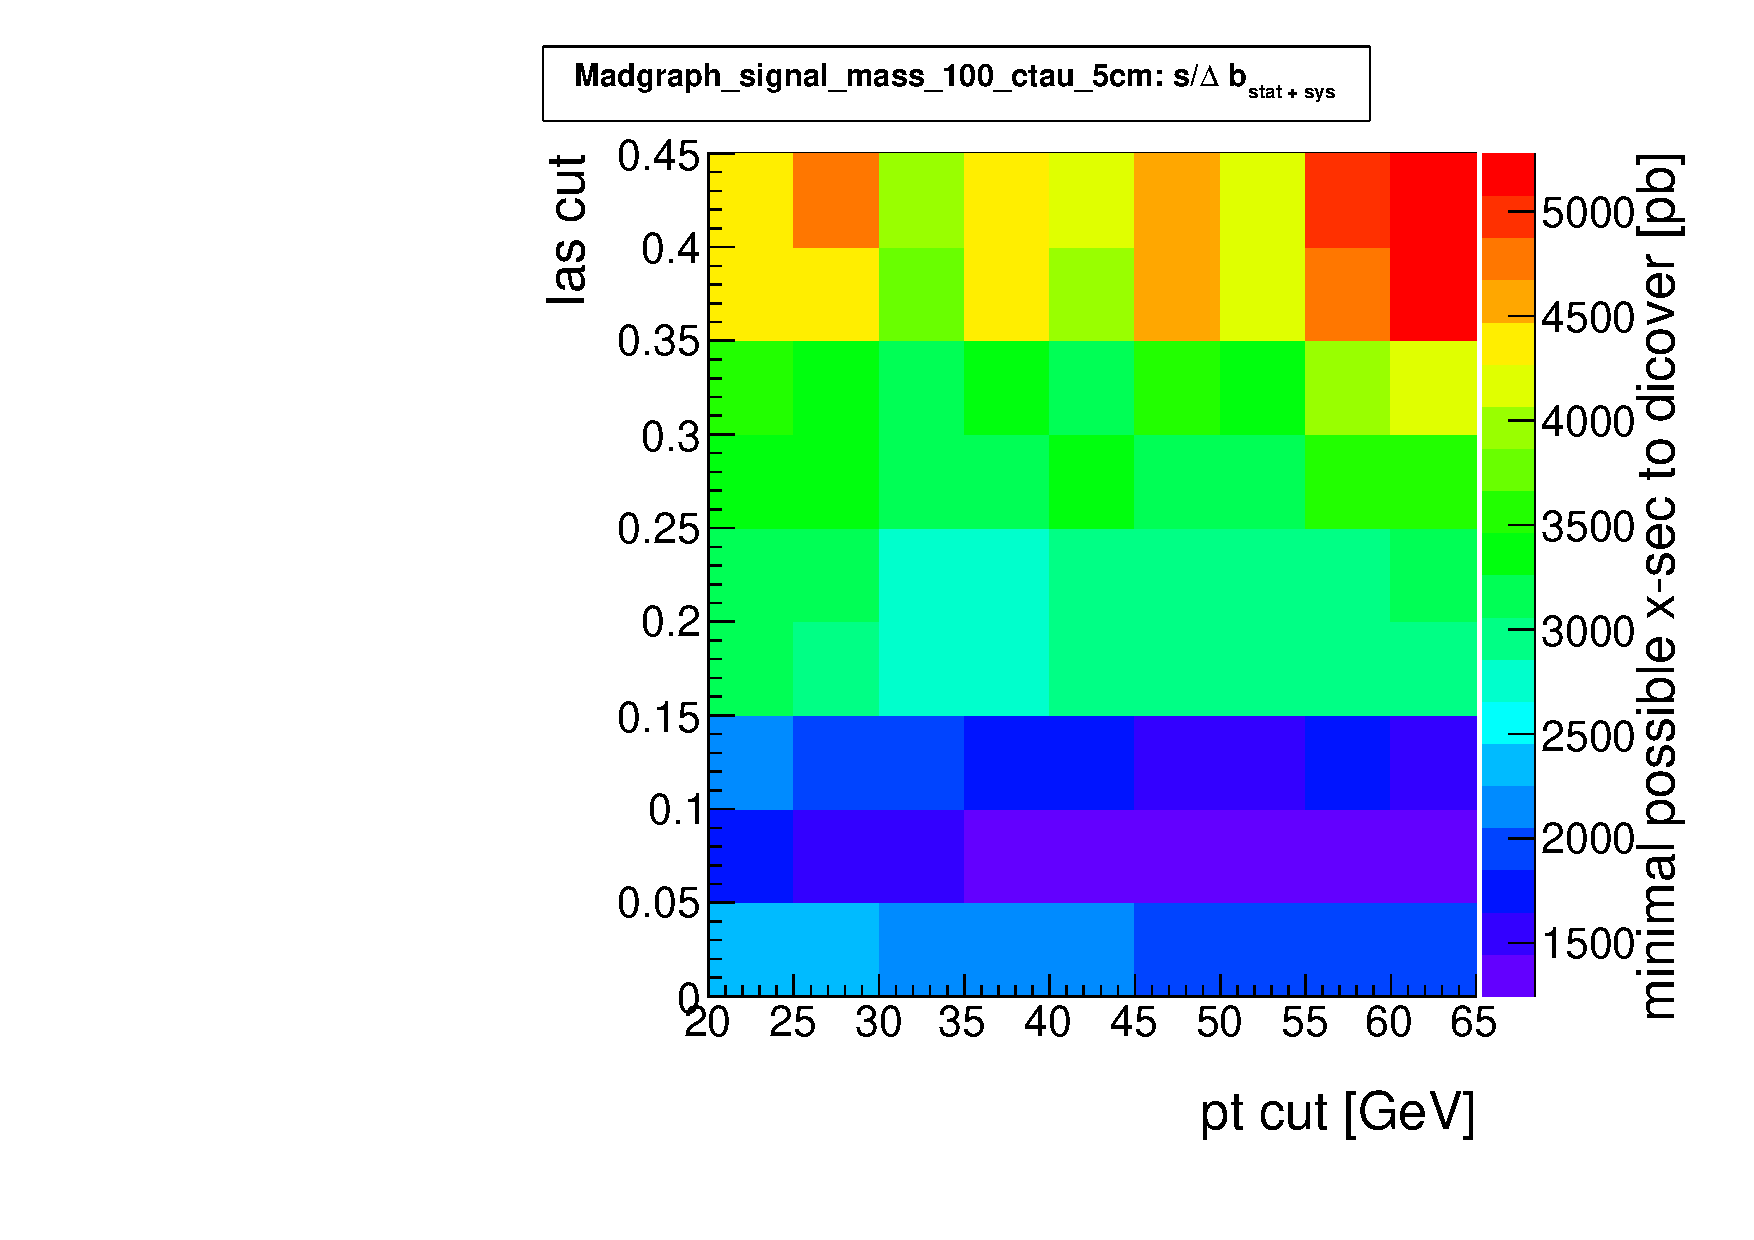
\includegraphics[width=0.49\textwidth]{figures/analysis/Optimisation/Madgraph_signal_mass_100_ctau_5cm_ECaloLe5_SOverDeltaBStatPlusSys.pdf} 
    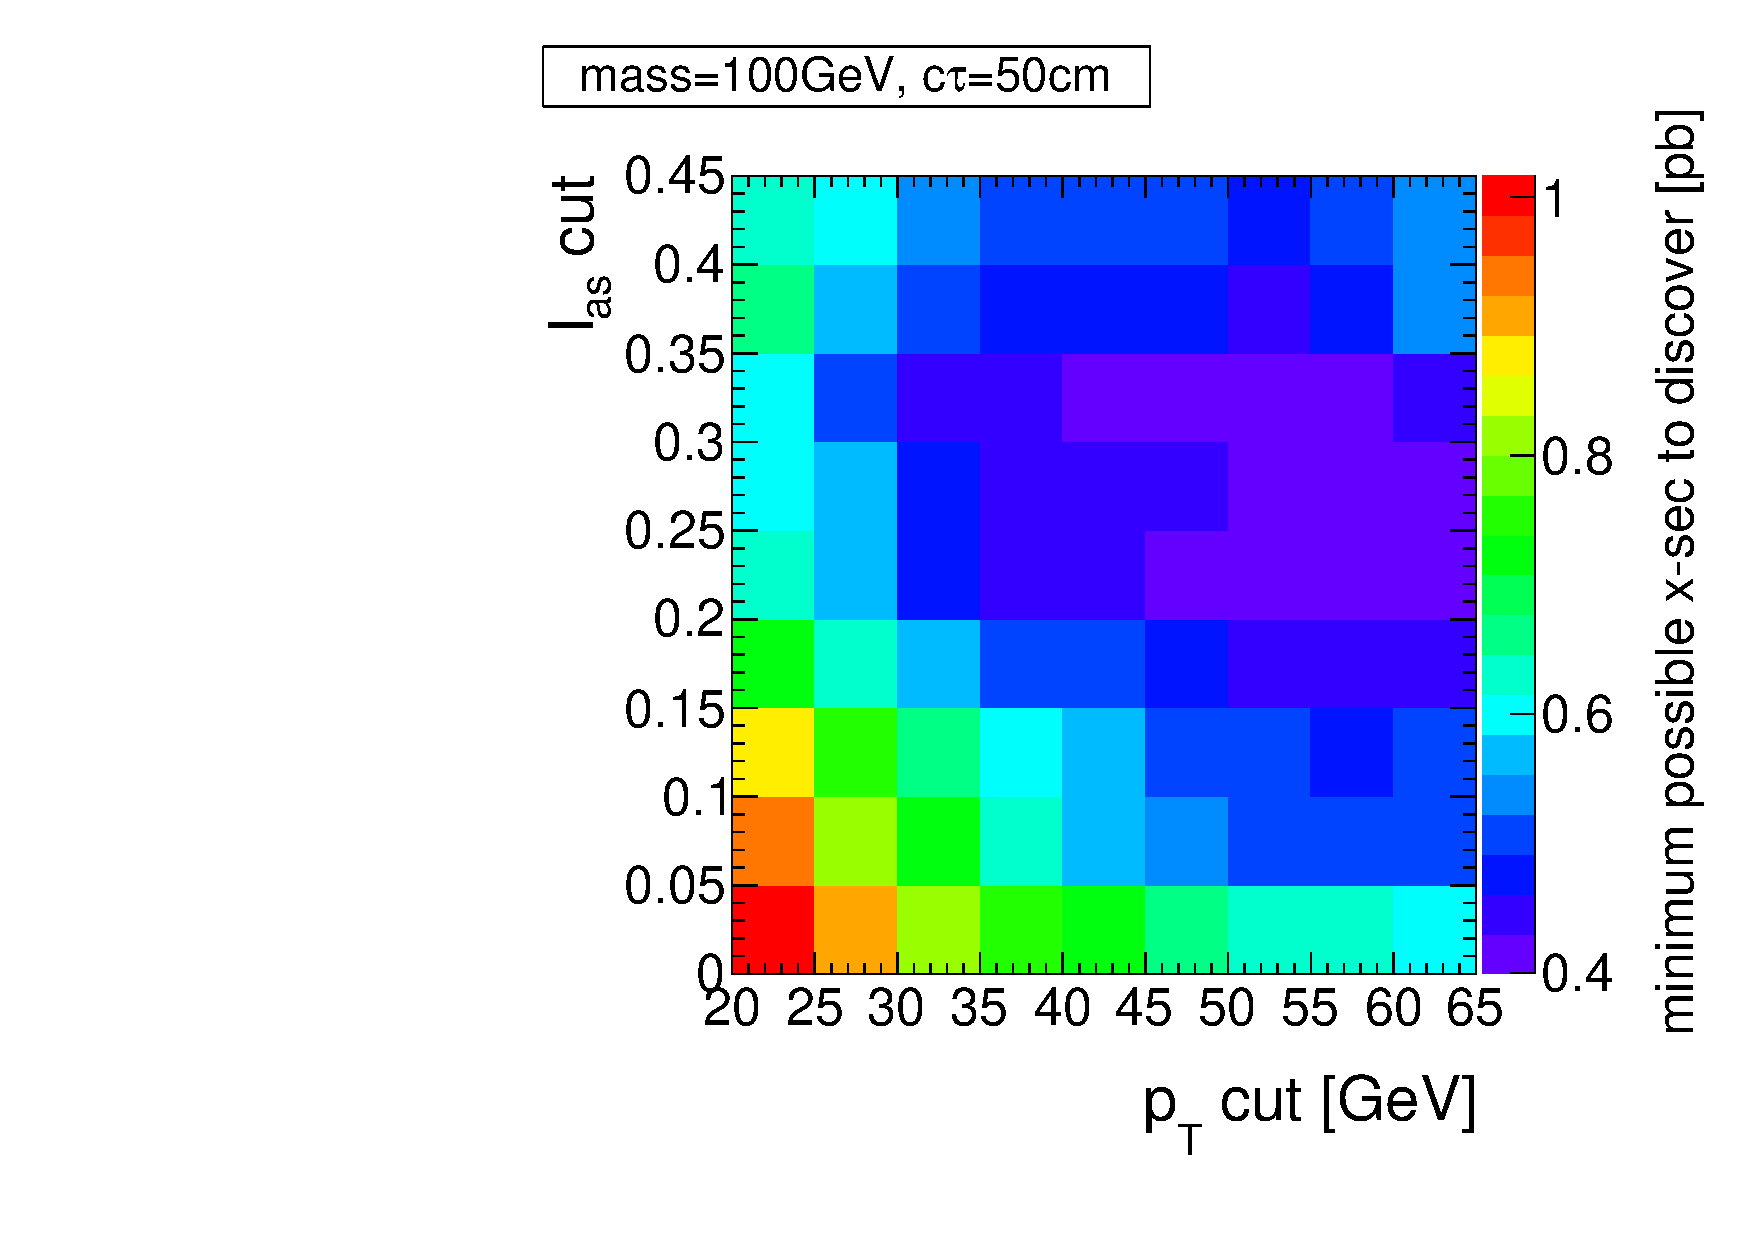
\includegraphics[width=0.49\textwidth]{figures/analysis/Optimisation/Madgraph_signal_mass_100_ctau_50cm_ECaloLe5_SOverDeltaBStatPlusSys.pdf}\\ 
    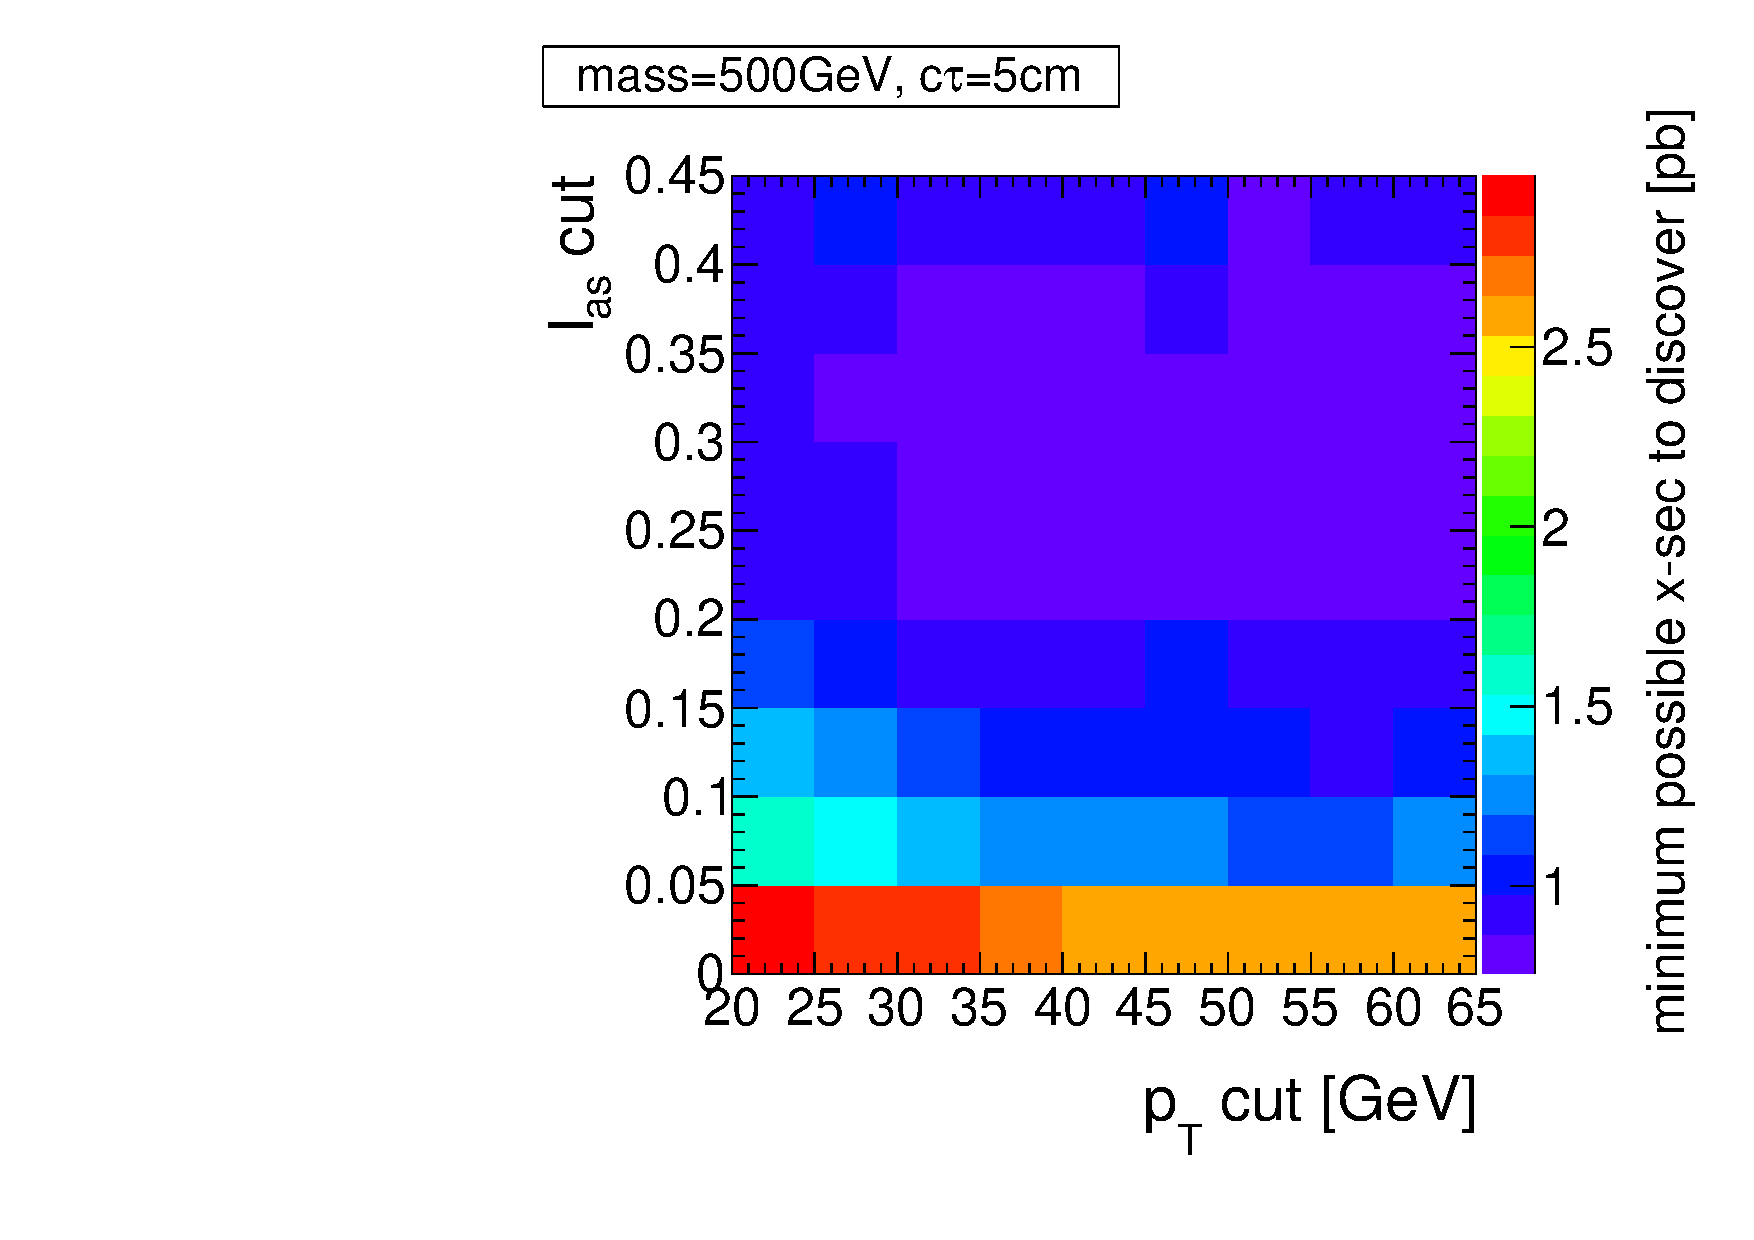
\includegraphics[width=0.49\textwidth]{figures/analysis/Optimisation/Madgraph_signal_mass_500_ctau_5cm_ECaloLe5_SOverDeltaBStatPlusSys.pdf}
    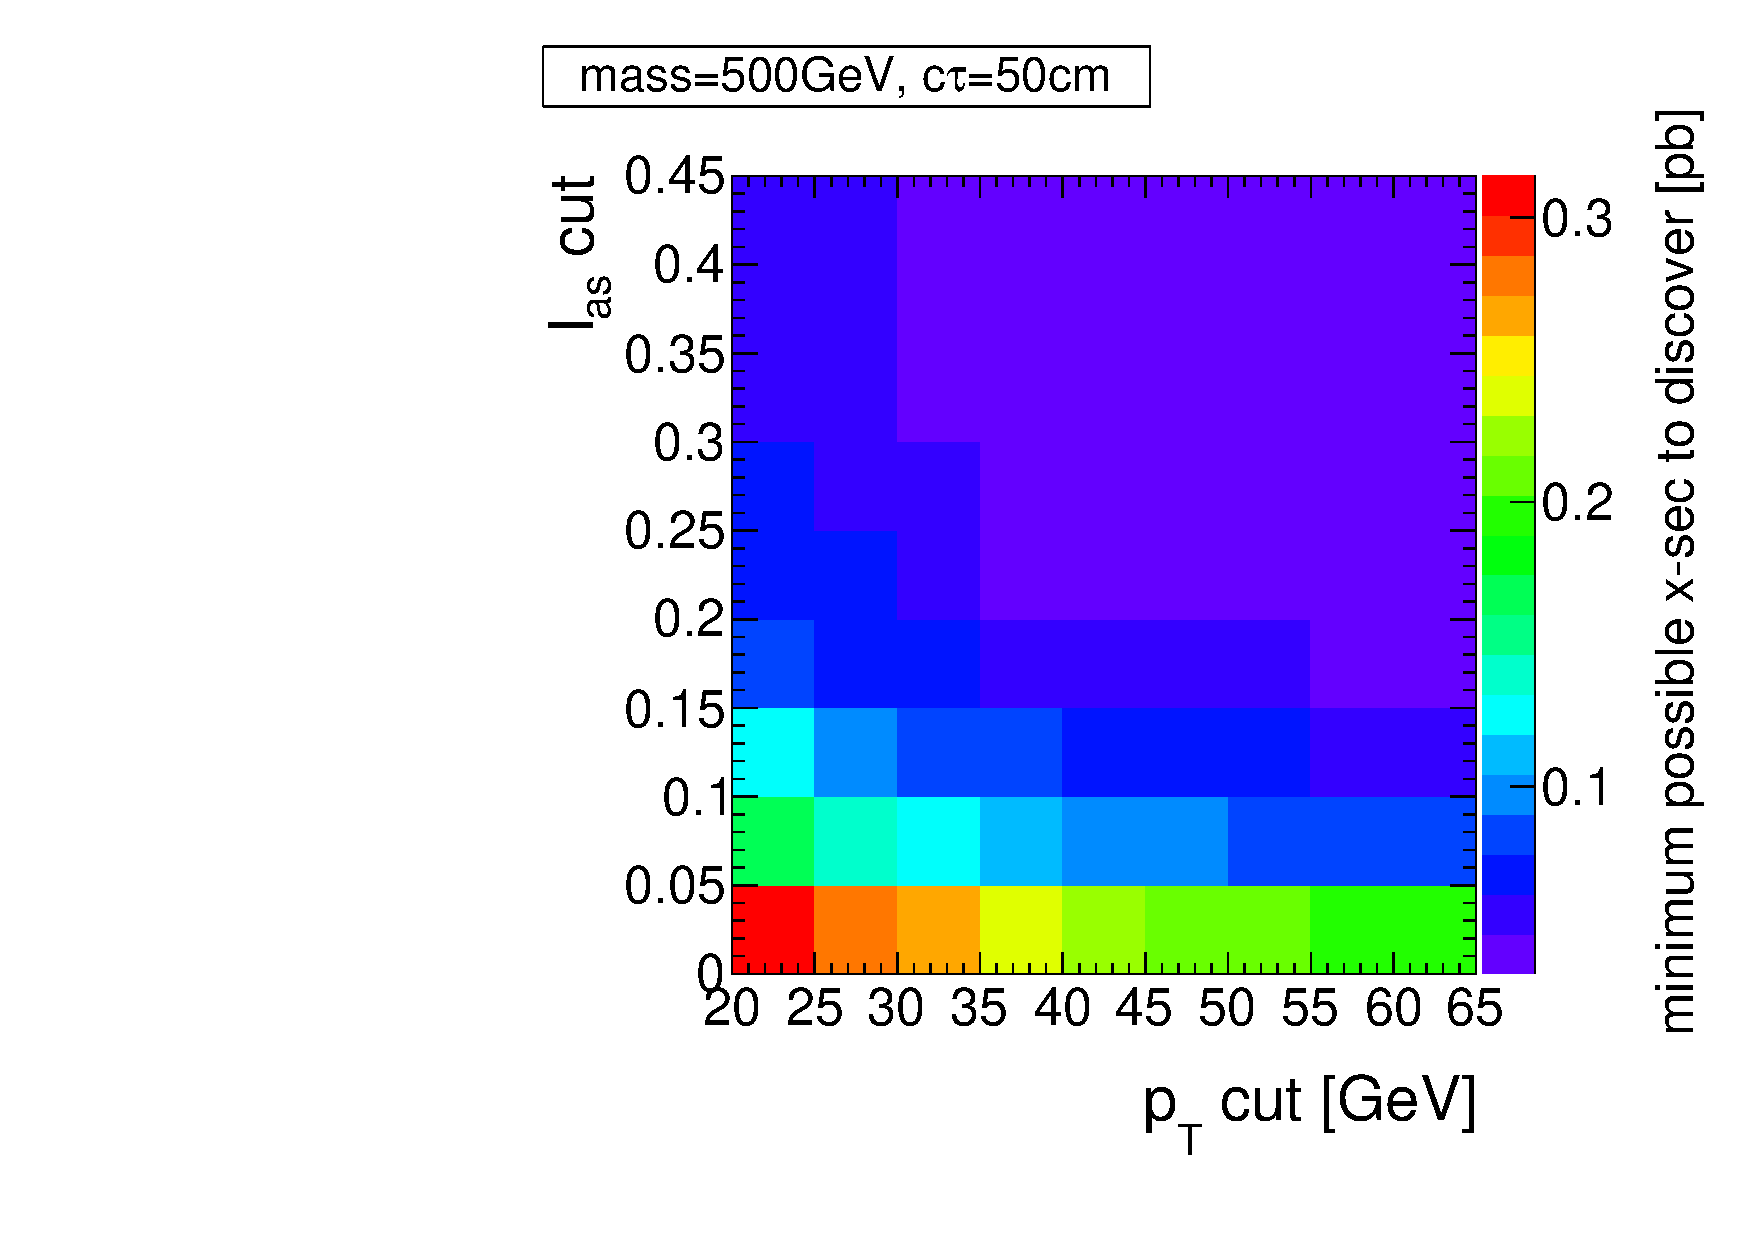
\includegraphics[width=0.49\textwidth]{figures/analysis/Optimisation/Madgraph_signal_mass_500_ctau_50cm_ECaloLe5_SOverDeltaBStatPlusSys.pdf} 
  \end{tabular}
  \caption{Minimum possible cross section that can be discovered with 5$\sigma$ significance in the $\ias-\pt$ plane for four different signal models.
           The systematic uncertainties are taken to be 20\% and 100\% for the fake and the leptonic background respectively.
           The uncertainty on the background arising from the limited size of the used samples are propagated consistently to the search optimisation.
           In Table~\ref{fig:optimisationApp} of Appendix~\ref{app:OptimisationApp}, the corresponding histograms of the background yield, the background uncertainty and the signal yield for the four signal models can be found.}
  \vspace{10pt}
  \label{fig:optimisation}
\end{figure}
Similar to the full optimisation, it can be seen that for low masses and low lifetimes, the highest search sensitivity is achieved by imposing rather soft selection cuts on \ias and \pt.
Optimising for higher lifetime pushes the optimal selection in \pt and \ias to larger values, where signal models with higher masses prefer even tighter \ias selection cuts than the corresponding lower mass signal model.
It can also be seen, that for low lifetimes, the \pt dependence of the search sensitivity is less pronounced than for long lifetimes.\\


Based on the optimisation, four different exclusive signal regions are defined in order to achieve an optimal coverage over a wide mass space and a high sensitivity for different lifetimes:
\begin{enumerate}[1.)]
\item $30\gev<\pt<50\gev$ and $0.05<\ias<0.3$
\item $\pt>50\gev$ and $0.05<\ias<0.3$
\item $30\gev<\pt<50\gev$ and $\ias>0.3$
\item $\pt>50\gev$ and $\ias>0.3$.
\end{enumerate}

The unblinded results of the search for highly ionising, short tracks are presented in the following chapter.
%%%%%%%%%%%%%%%%%%%%%%%%%%%%%%%%%%%%%%%%%%%%%%%%%%%%%%%%%%%%%%%%%%%%%%%%%%%%%%%%%%%%%%%%%%%%%%%%%%%%%%%%%%%%%%%%%%%%%%%%%%%%%%%%%%%%%%%%%%%%%%%%%%%%%%%%%%%%%%%%%%%%%%%
%%%%%%%%%%%%%%%%%%%%%%%%%%%%%%%%%%%%%%%%%%%%%%%%%%%%%%%%%%%%%%%%%%%%%%%%%%%%%%%%%%%%%%%%%%%%%%%%%%%%%%%%%%%%%%%%%%%%%%%%%%%%%%%%%%%%%%%%%%%%%%%%%%%%%%%%%%%%%%%%%%%%%%%
\FloatBarrier
\chapter{Results}
\label{sec:Results}

After developing the methods of the background estimation for all different background sources and their corresponding systematic uncertainties (all explained in Section~\ref{sec:BackgroundEstimation}), 
the search is performed in four exclusive signal regions with 19.7\fbinv of data collected at a centre-of-mass energy of $\sqrt{s} = 8\tev$ at the CMS experiment.
The predicted number of events for the fake and the leptonic background in the four signal regions is depicted in Table~\ref{tab:BackgroundPrediction}.
\renewcommand{\arraystretch}{1.5}
\begin{table}[!t]
\centering
\caption{Background prediction in the four exclusive signal regions for the fake and the leptonic background.}
\label{tab:BackgroundPrediction}
\makebox[0.99\textwidth]{
\begin{tabular}{l |c| c }
\multicolumn{3}{c}{} \\
\toprule
Signal region                                & Fake Bkg                                             & Leptonic Bkg  \\
\midrule
$\pt: 30-50\gev$ / $\ias:0.05-0.30$          & 19.11 $^{+ 2.61} _{- 2.61}$ (stat) $\pm$ 9.35 (sys)      & 0.00 $^{+ 2.58} _{- 0.00}$ (stat) $\pm$ 0.00 (sys) \\
$\pt: 50-\infty\gev$ / $\ias:0.05-0.30$      & 22.21 $^{+ 3.60} _{- 3.60}$ (stat) $\pm$ 8.78 (sys)      & 2.17 $^{+ 2.99} _{- 1.34}$ (stat) $\pm$ 1.65 (sys) \\
$\pt: 30-50\gev$ / $\ias:0.30-1.00$          & 2.49 $^{+ 0.85} _{- 0.85}$ (stat) $\pm$ 1.98 (sys)       & 0.00 $^{+ 0.22} _{- 0.00}$ (stat) $\pm$ 0.00 (sys) \\
$\pt: 50-\infty\gev$ / $\ias:0.30-1.00$      & 2.52 $^{+ 1.14} _{- 1.14}$ (stat) $\pm$ 1.27 (sys)       & 0.04 $^{+ 0.30} _{- 0.03}$ (stat) $\pm$ 0.03 (sys) \\
\bottomrule
\multicolumn{3}{c}{}\\
\end{tabular}}
\end{table}
It can be seen, that fake tracks are by far the dominant background to this search.
The leptonic background contributes only in one signal region to the total background with a share of about 10\%.

Finally, the comparison between the predicted number of events and the number of observed events is shown in Fig.~\ref{fig:FinalResult}.
\begin{figure}[!b]
  \centering 
  \vspace{55pt}
  \begin{tabular}{c}
    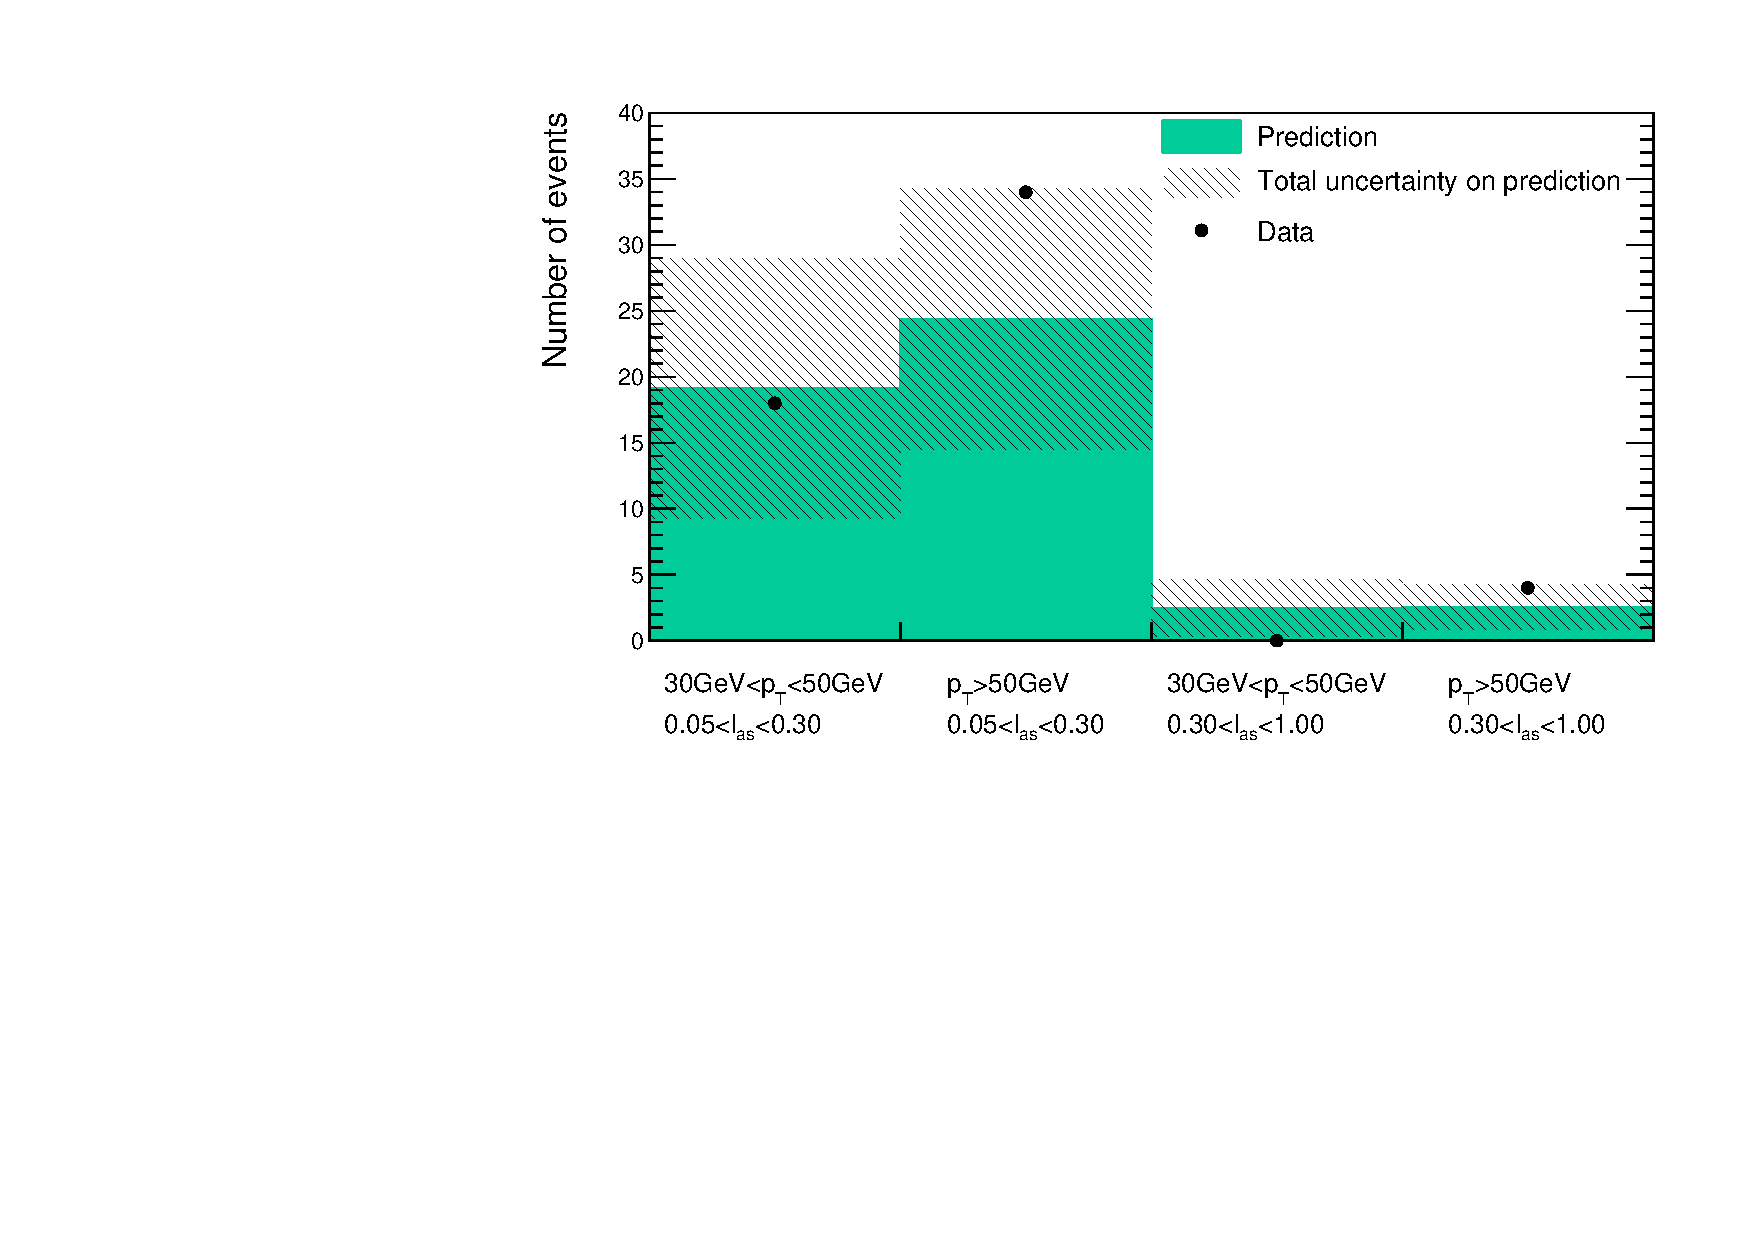
\includegraphics[width=0.99\textwidth]{figures/analysis/Results/FinalResultPlot.pdf} 
  \end{tabular}
  \caption{Number of predicted (green area) and observed (black dots) events for the four different signal regions. The hashed area represents the total uncertainty on the background prediction.}
  \label{fig:FinalResult}
\end{figure} 
Additionally, the corresponding numbers of predicted and observed events can be found in Table~\ref{tab:FinalResult}.
\renewcommand{\arraystretch}{1.5}
\begin{table}[!t]
\centering
\caption{Number of predicted and observed events for the four different signal regions.}
\label{tab:FinalResult}
\makebox[0.99\textwidth]{
\begin{tabular}{l |c| c}
\multicolumn{3}{c}{} \\
\toprule
Signal region                         & Prediction                                              & Observation  \\
\midrule
$\pt: 30-50\gev$ / $\ias:0.05-0.30$      & 19.11 $^{+ 3.67} _{- 2.61}$ (stat) $\pm$ 9.35 (sys)         & 18           \\
$\pt: 50-\infty\gev$ / $\ias:0.05-0.30$  & 24.38 $^{+ 4.68} _{- 3.84}$ (stat) $\pm$ 8.93 (sys)         & 34           \\
$\pt: 30-50\gev$ / $\ias:0.30-1.00$     & 2.49 $^{+ 0.87} _{- 0.85}$ (stat) $\pm$ 1.98 (sys)          & 0            \\
$\pt: 50-\infty\gev$ / $\ias:0.30-1.00$ & 2.57 $^{+ 1.18} _{- 1.14}$ (stat) $\pm$ 1.27 (sys)          & 4            \\
\bottomrule
\multicolumn{3}{c}{} \\
\end{tabular}}
\end{table}
The event yields observed in data after each selection requirement for the four signal regions are listed in Table~\ref{tab:CutflowData} in Appendix~\ref{app:cutflow}.

The results are compatible with the Standard Model background within 1$\sigma$ uncertainties in all four signal regions.
No excess above the SM prediction is observed in either of the four signal regions.
Thus, no evidence for physics beyond the Standard Model could be found.

Therefore, in the following section these results will be used to constrain the parameter space of supersymmetric models with almost mass degenerate charginos and neutralinos.
%\renewcommand{\arraystretch}{1.5}
%\begin{table}[!h]
%\centering
%\caption{Background prediction from the four different background sources: Fakes, taus, muons and electrons.}
%\label{tab:FinalResult}
%\makebox[0.99\textwidth]{
%\begin{tabular}{l |c| c | c| c}
%\multicolumn{3}{c}{} \\
%\toprule
%Signal region                         & Fakes   & Taus  & Muons & Electrons  \\
%\midrule
%$30\gev<\pt<50\gev$ / $0.05<\ias<0.3$ & 19.11 $^{+ 2.61} _{- 2.61}$ (stat) $\pm$ 9.35 (sys)      & 0.00 $^{+ 0.87} _{- 0.00}$ (stat) $\pm$ 0.00 (sys) & 0.00 $^{+ 0.22} _{- 0.00}$ (stat) $\pm$ 0.00 (sys) & 0.00 $^{+ 2.42} _{- 0.00}$ (stat) $\pm$ 0.00 (sys)                           \\
%$\pt>50\gev$        / $0.05<\ias<0.3$ & 22.21 $^{+ 3.60} _{- 3.60}$ (stat) $\pm$ 8.78 (sys)      & 0.00 $^{+ 0.33} _{- 0.00}$ (stat) $\pm$ 0.00 (sys) & 0.00 $^{+ 0.29} _{- 0.00}$ (stat) $\pm$ 0.00 (sys) & 2.17 $^{+ 2.96} _{- 1.34}$ (stat) $\pm$ 1.65 (sys)                             \\
%$30\gev<\pt<50\gev$ / $\ias>0.3$      & 2.49 $^{+ 0.85} _{- 0.85}$ (stat) $\pm$ 1.98 (sys)       & 0.00 $^{+ 0.01} _{- 0.00}$ (stat) $\pm$ 0.00 (sys) & 0.00 $^{+ 0.22} _{- 0.00}$ (stat) $\pm$ 0.00 (sys) & 0.00 $^{+ 0.05} _{- 0.00}$ (stat) $\pm$ 0.00 (sys)                      \\
%$\pt>50\gev$        / $\ias>0.3$      & 2.52 $^{+ 1.14} _{- 1.14}$ (stat) $\pm$ 1.27 (sys)       & 0.00 $^{+ 0.00} _{- 0.00}$ (stat) $\pm$ 0.00 (sys) & 0.00 $^{+ 0.29} _{- 0.00}$ (stat) $\pm$ 0.00 (sys) & 0.04 $^{+ 0.06} _{- 0.03}$ (stat) $\pm$ 0.03 (sys)                      \\
%\bottomrule
%\multicolumn{3}{c}{} \\
%\end{tabular}}
%\end{table}


%%%%%%%%%%%%%%%%%%%%%%%%%%%%%%%%%%%%%%%%%%%%%%%%%%%%%%%%%%%%%%%%%%%%%%%%%%%%%%%%%%%%%%%%%%%%%%%%%%%%%%%%%%%%%%%%%%%%%%%%%%%%%%%%%%%%%%%%%%%%%%%%%%%%%%%%%%%%%%%%%%%%%%%
%%%%%%%%%%%%%%%%%%%%%%%%%%%%%%%%%%%%%%%%%%%%%%%%%%%%%%%%%%%%%%%%%%%%%%%%%%%%%%%%%%%%%%%%%%%%%%%%%%%%%%%%%%%%%%%%%%%%%%%%%%%%%%%%%%%%%%%%%%%%%%%%%%%%%%%%%%%%%%%%%%%%%%%
\chapter{Interpretation}
\label{sec:Interpretation}
In order to interpret the result of the search in the context of supersymmetric models with almost mass degenerate charginos and neutralinos, sources of systematic uncertainties on the number of selected signal events must be identified and quantified.
The interpretation will then be done with statistical methods that allow for the exclusion of parts of the supersymmetric parameter space on a 95\% confidence level.

\section{Systematic uncertainties of simulated signal samples}
The systematic uncertainties on the number of signal events in the four signal regions are mainly caused by uncertainties on the quality of the simulation.
This influences the signal efficiency of each selection requirement in this analysis.
Furthermore, an uncertainty on the overall number of events is caused by the uncertainty on the integrated luminosity recorded in 2012 at CMS and the theoretical signal cross sections.

All systematic uncertainties are estimated for each signal model and each search bin separately.
In the following, the sources of systematic uncertainties are discussed and the minimum and maximum value of the corresponding uncertainty is given.

\subsection*{Uncertainty on the theoretical cross section}
The theoretical cross sections of $\chipm\chimp$ and $\chipm\chiO$ production at a centre-of-mass energy of 8\tev are taken from~\cite{bib:SignalCrossSection_2012,bib:SignalCrossSection_2013}.
The corresponding theoretical uncertainties range between $4.5-12.1\%$.

\subsection*{Luminosity uncertainty}
The integrated luminosity recorded at CMS during the year 2012 is measured by counting of pixel clusters during the crossing of two bunches (zero-bias event).
A detailed explanation of this method and the corresponding total uncertainty of 2.6\% can be found in \cite{bib:CMS:Lumi_PAS}.

\subsection*{Uncertainty on the simulation of initial state radiation}
Initial state radiation affects the transverse momentum distribution of the 2-particle system, $\pt\left(p_1^{\mu} + p_2^{\mu} \right)$, in a 2-body decay.
Differences between data and simulation of ISR are taken into account by reweighting the simulated events, such that the simulated transverse momentum distribution matches the measured distribution in data. 
The weights and associated systematic uncertainties are determined in~\cite{bib:CMS:ISR_AN} by comparing simulated and observed \pt distributions of $Z$ and $\bar{t}t$ events.
These weights are applied to the simulated $\chipm\chimp$ and $\chipm\chiO$ events.
To account for the systematic uncertainties on the reweighting procedure, the event weights are varied up and down by up to 25\% according to~\cite{bib:CMS:ISR_AN} depending on the $\pt^{\chi_1\chi_2}$.
The resulting uncertainty on the ISR simulation is between $9.2-12.6\%$.

\subsection*{Uncertainty on the simulation of the trigger efficiency}
The HLTMonoCentralPFJet80\_PFMETnoMu105\_NHEF0p95 trigger with the higher MET threshold of 105\gev active in Run\,C and Run\,D during 2012 was not available in the simulated signal samples.
It is therefore emulated using HLT trigger information. 
More details on the emulation of this trigger can be found in Appendix~\ref{app:TriggerEmulation}.

The trigger uncertainty is assessed by comparing data-simulation differences of the trigger efficiency.
This uncertainty has been quantified within~\cite{bib:CMS:DT_Thesis,bib:CMS:DT_8TeV_AN} by comparing simulated and measured trigger turn-on curves and determining weights for simulated events such that simulated and observed turn-on curves are compatible.
These event weights are applied on the simulated signal samples in this analysis and lead to changes in the signal prediction of $1.9-4.4\%$.

\subsection*{Uncertainty on the jet energy scale}
The transverse momentum of all jets is corrected for non-uniformities in the energy response as a function of the jet $\eta$ and \pt and for data-simulation differences~\cite{bib:CMS:JME_PAS}.
The uncertainty on the jet energy scale (JES) is neatly described and quantified in~\cite{bib:CMS:JME_PAS}. 
It arises from uncertainties on the jet response in data including jet fragmentation, jet flavor composition, etc..
The JES correction is applied as a multiplicand on each jet's transverse momentum contained in an event.
The corresponding systematic uncertainty is assessed by an up- and downward variation of the correction factor within 1\,$\sigma$.
The resulting uncertainties are of minor importance and range between $0.4-3.1\%$.

\subsection*{Uncertainty on the jet energy resolution}
The jet energy resolution (JER) is smaller in simulation than in measured data (see Part~\ref{FIXME}). 
In order to take these differences into account, the simulated jet energy response is smeared to match the measured response.
The systematic uncertainty on the smearing factors is estimated in~\cite{bib:CMS:JME_PAS,bib:Kristin_Thesis}.
It covers the uncertainty on JER in data, including the JES uncertainty, uncertainties arising from out-of-cone showering etc.~\cite{bib:CMS:JME_PAS,bib:Kristin_Thesis}.
The resulting uncertainty on the signal efficiency in this study is between $0.1-2.0\%$ and therefore almost negligible.

\subsection*{Uncertainty on the simulation of the parton distribution functions}
The parton distribution function (PDF) used for the simulation of proton-proton collisions is provided by the \cteq group~\cite{Pumplin:2002vw} (see Section~\ref{FIXME} for more information about PDFs).
In~\cite{Pumplin:2002vw}, a detailed description of the determination of a parton distribution function and its uncertainties is given.
Practically, the estimation of the PDF uncertainty is done by the application of 44 different sets of event weights which take into account 22 different sources of uncertainties~\cite{Botje:2011sn,bib:PDF_practical} 
(up and down variations lead to a factor of 2).
The sources correspond inter alia to uncertainties in the single distributions of gluons, up/down-quarks, etc, with the gluon distribution being by far the largest source of uncertainty.

The resulting uncertainties on the signal efficiency for this search are between $2.6-6.8\%$.

\subsection*{Uncertainty of the pileup reweighting}
The distribution of the number of primary vertices in simulation is reweighted to match the measured distribution in data.
The number of primary vertices in data is determined by the luminosity of each bunch-crossing times the proton-proton inelastic cross section which is 69.4\mb~\cite{bib:CMS:PileupUtilities}.
The uncertainty on the number of interactions thus consists of the uncertainty on the luminosity and the uncertainty on the cross section.
To cover both sources, a variation of the inelastic cross section by plus/minus 5\% is done according to the recommendation by~\cite{bib:CMS:PileupSysUnc}.

For most of the signal models and signal regions, the signal efficiency is only affected by less than 1\% by the pileup reweighting uncertainty.
If the statistical precision of the signal prediction in a specific search bin is low, the uncertainty can become significantly larger.
However, the search sensitivity is always driven by search bins with high signal content so that large values of this uncertainty have no effect on the overall search sensitivity.

\subsection*{Uncertainty on the simulation of the calorimeter isolation}
The uncertainty on the simulation of the calorimeter isolation \ecalo is estimated by comparing simulated and measured selection efficiencies of $\ecalo<5\gev$ in the fake enriched control sample \fakeCR.
The fake enriched control region is well suited for this estimation, as fake tracks are also expected to deposit only a low amount of energy in the calorimeters.
The selection efficiency in data is higher than in simulation in both \pt bins of $30-50\gev$ and $50-\infty\gev$, resulting in an uncertainty of 12.1\% and 3.0\% respectively.

\subsection*{Uncertainty on the simulation of missing middle/inner hits}
The uncertainty on the simulation of the number of missing inner and middle hits is assessed by comparing the probability in simulation and data of passing the selection requirements of $N_{\text{miss}}^{\text{middle/inner}}=0$
of a candidate track in the muon-veto inverted control region. 
This control region is particularly suitable because muons are not expected to have intrinsic sources of missing hits, as \eg pions or electrons have.
Pions can interact nuclearly with the tracker material and electrons can have sizable radiative losses, such that both can change direction or don't deposit energy in a tracker layer.
For muons, on the other hand, sources of missing inner and middle hits are mainly algorithmic~\cite{bib:CMS:DT_Thesis,bib:CMS:DT_8TeV_AN}, 
making them very similar to the algorithmic sources of missing inner/middle hits for chargino tracks.

The uncertainty is estimated as the relative difference of the cut selection efficiency of $N_{\text{miss}}^{\text{middle/inner}}=0$ in data and simulation.
The selection efficiency is always higher in simulation, resulting in systematic uncertainties of around 3.5\% for the simulation of $N_{\text{miss}}^{\text{inner}}=0$ and around 2.2\% for $N_{\text{miss}}^{\text{middle}}=0$.
The uncertainties are of very similar size in the signal regions with different \pt.
No \ias dependence is considered.

\subsection*{Uncertainty on the simulation of \ias}
An uncertainty on the simulation of \ias needs to be estimated in order to account for possible data-simulation differences for highly ionising particles.
The estimation of the \ias uncertainty is done following the methodology in~\cite{bib:CMS:HSCP_8TeV,bib:CMS:HSCP_8TeV_AN}.
The \ias uncertainty can be assessed by comparing data and simulation differences of slow protons.
Slow protons are highly ionising and can thus be used to determine the uncertainty in the high \ias region.

In order to select slow protons, high quality tracks with a momentum smaller than 2.5\gev are selected.
The \ias versus momentum distribution for the selected tracks is shown in Fig.~\ref{fig:IasVsMomentum}.
The kaon, proton, and in data also the deuteron line is visible.
\begin{figure}[!h]
  \centering 
  \begin{tabular}{c}
    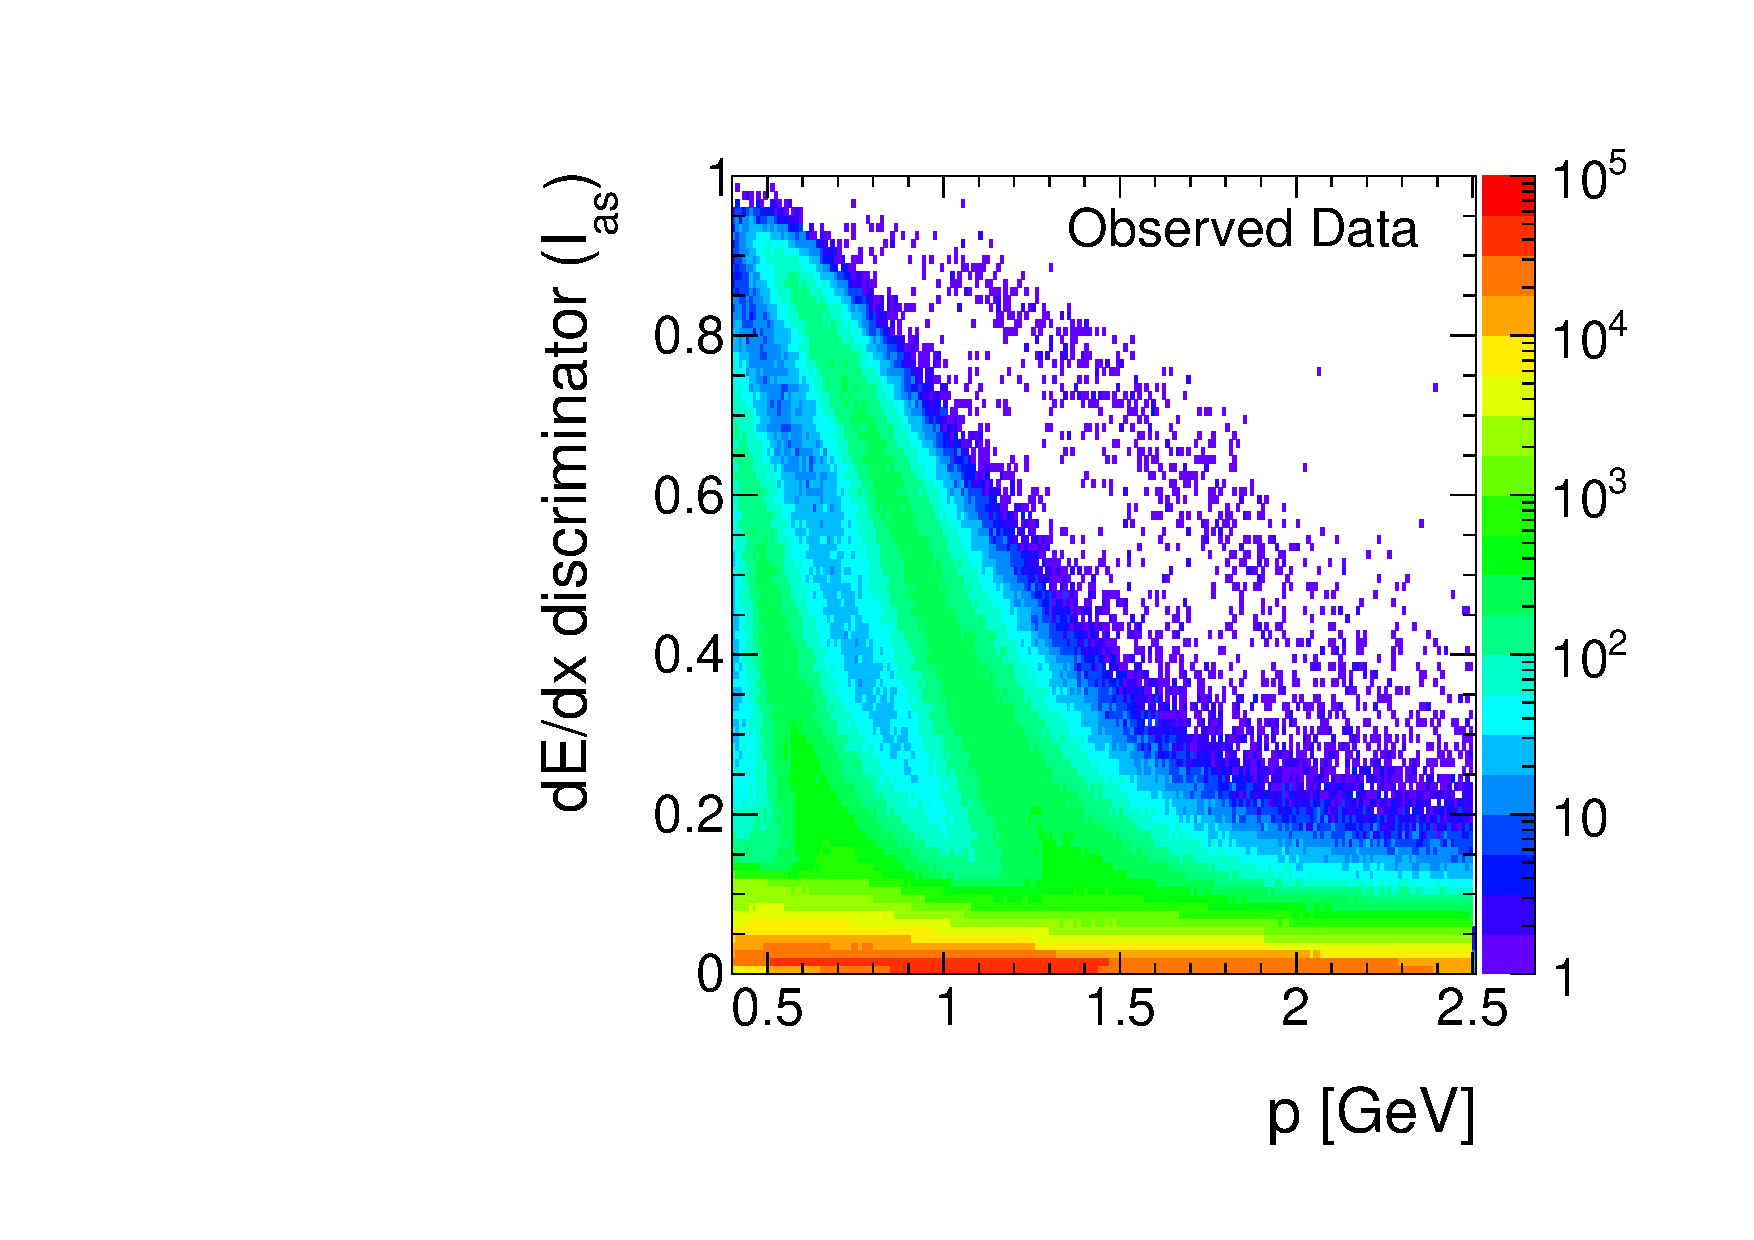
\includegraphics[width=0.49\textwidth]{figures/analysis/Interpretation/IasP_Data.pdf} 
    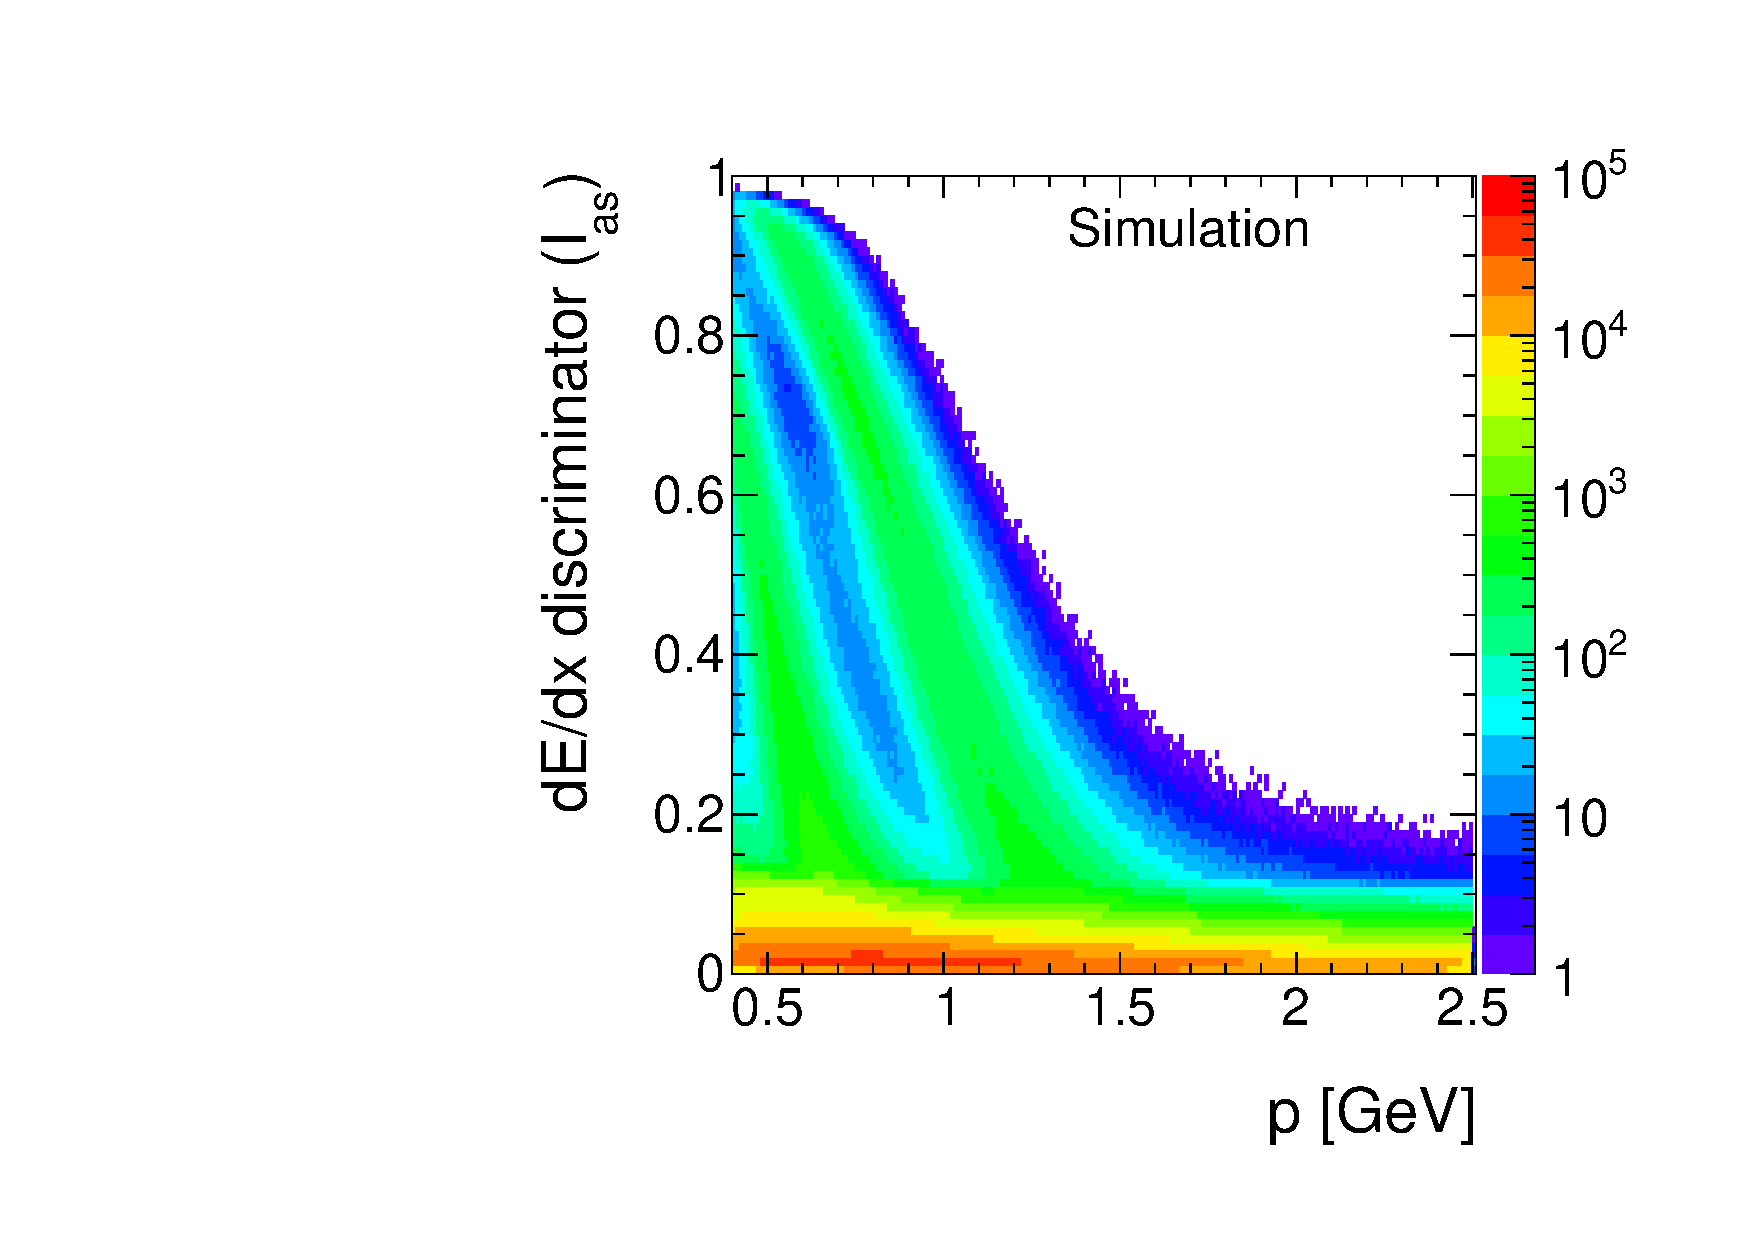
\includegraphics[width=0.49\textwidth]{figures/analysis/Interpretation/IasP_MC.pdf}
  \end{tabular}
  \caption{\ias versus momentum for good quality tracks with at least eight hits in observed data (left) and simulation (right).
           The kaon and proton line are visible in both datasets. The deuteron line is only visible in data, as deuteron's are not simulated.}
  \label{fig:IasVsMomentum}
\end{figure} 
Two different slices in the momentum are extracted where the proton line is contained: p between $0.80-0.85\gev$ and $0.95-1.00\gev$.
A Gaussian function is fitted to the proton peak and the maximum difference of the mean of the fitted Gaussian between simulation and observed data is taken as systematic uncertainty.
The \ias distribution for the two momentum ranges with the Gaussian fit is depicted in Fig.~\ref{fig:IasSlowProtons}.
\begin{figure}[!h]
  \centering 
  \begin{tabular}{c}
    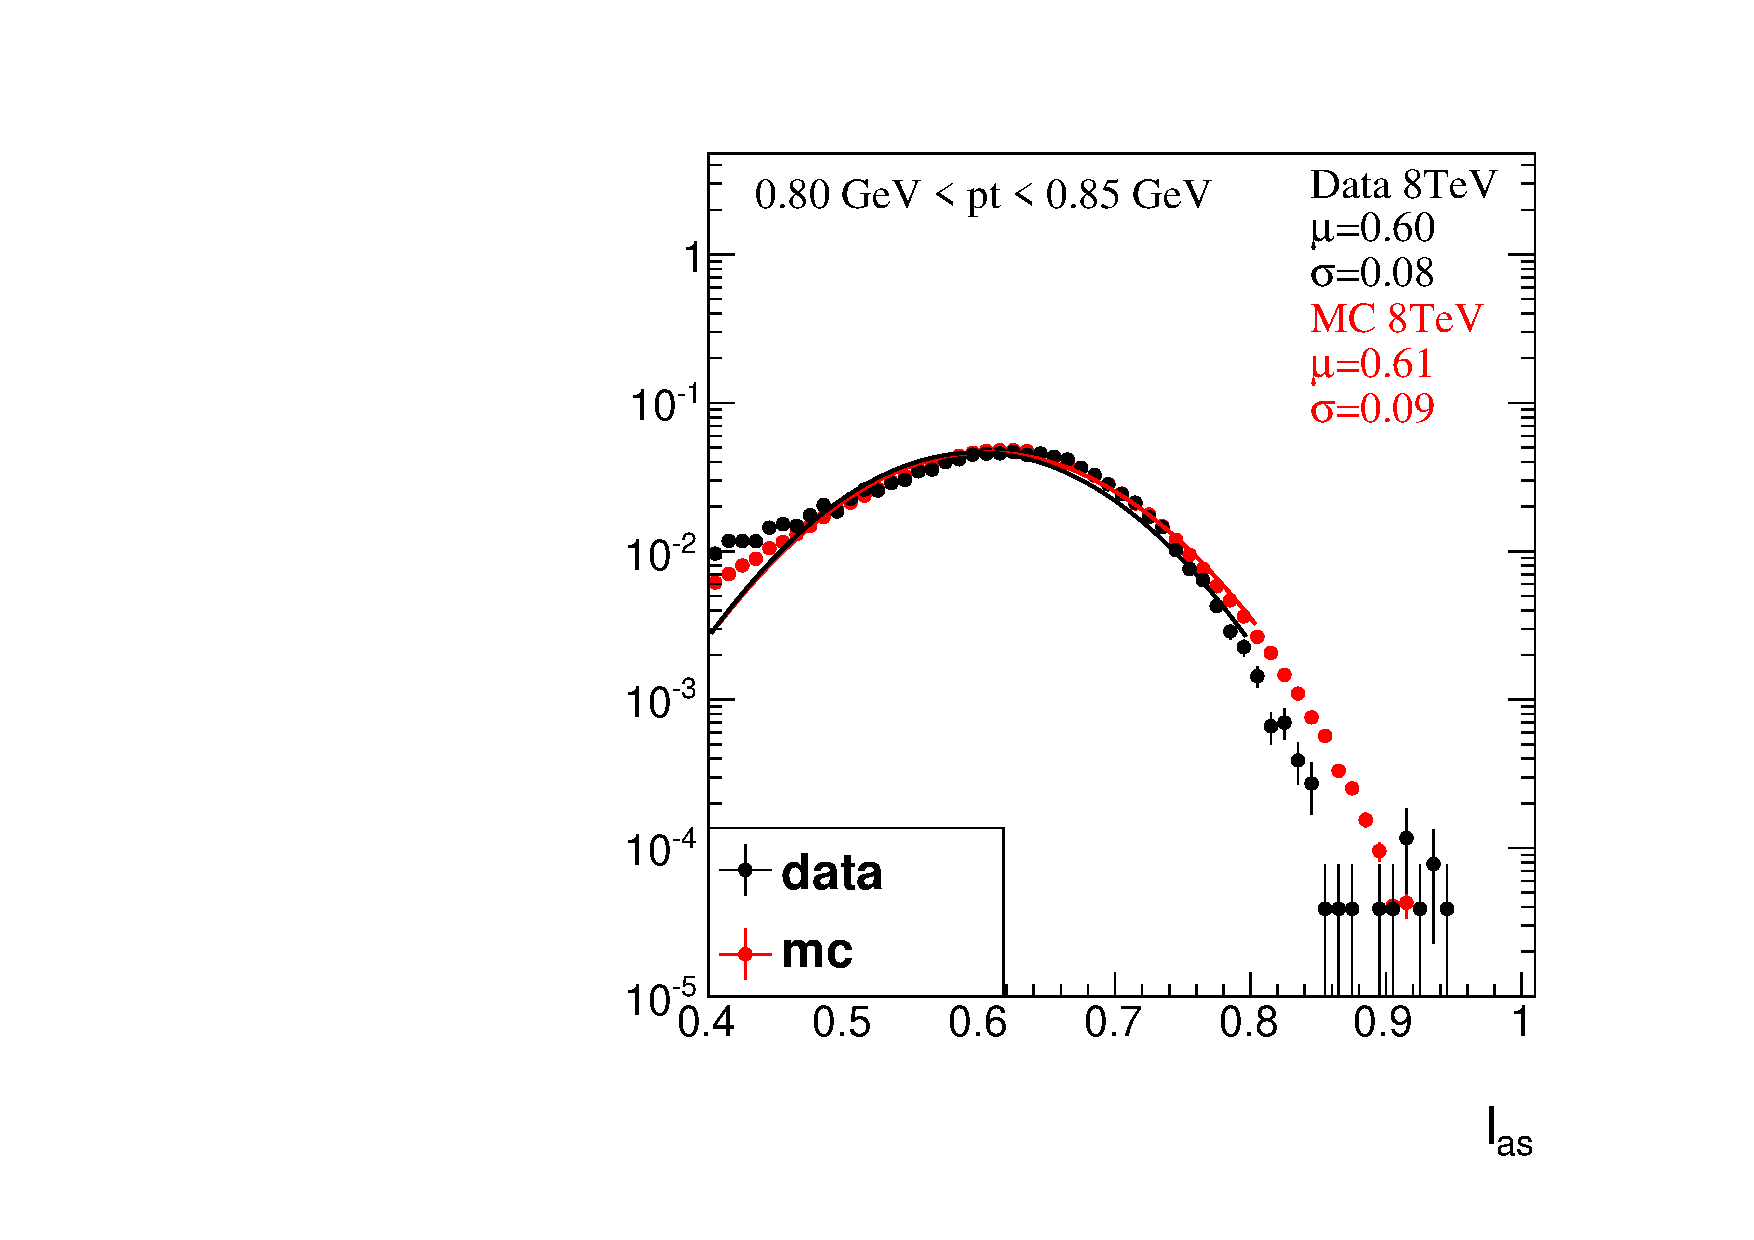
\includegraphics[width=0.49\textwidth]{figures/analysis/Interpretation/hIas_analysis_2015_11_30_ForThesis_ptmin0p80_ptmax0p85.pdf} 
    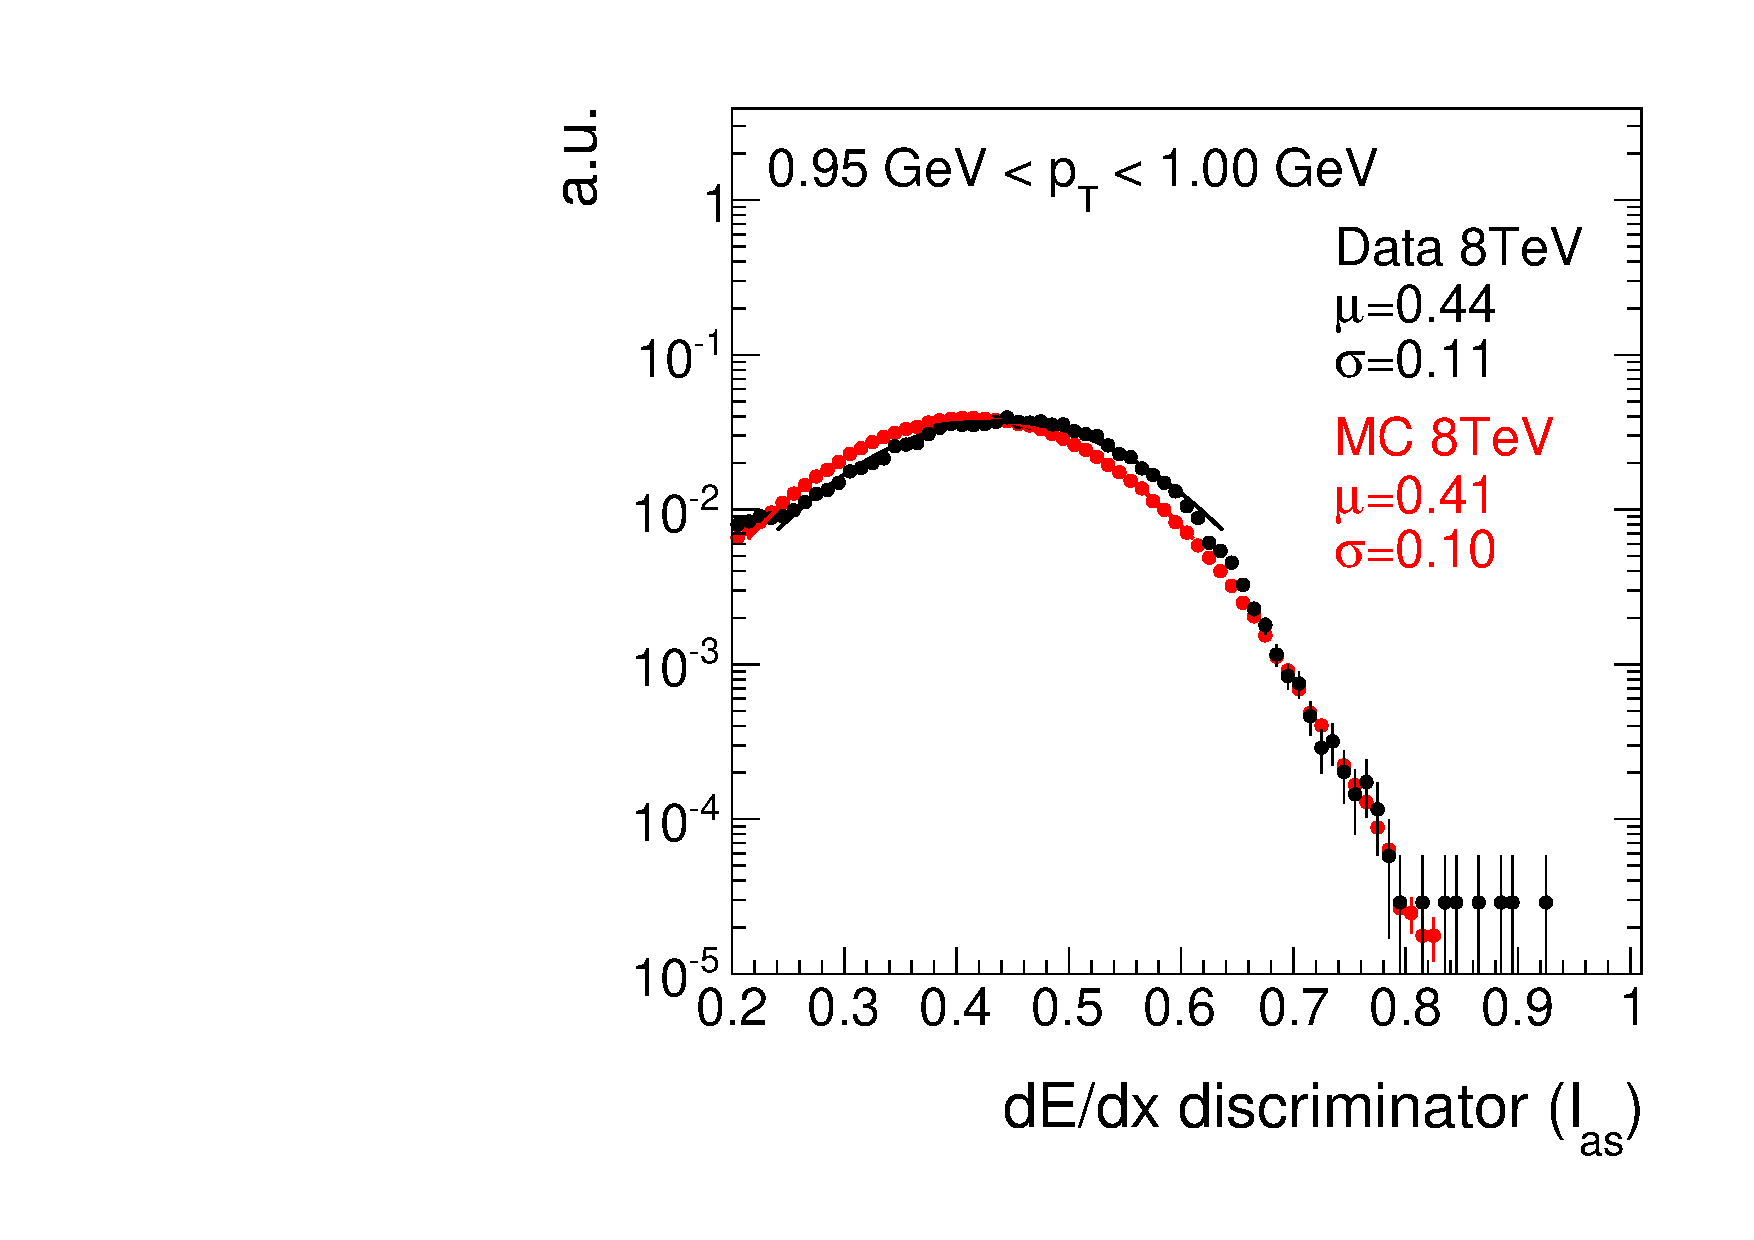
\includegraphics[width=0.49\textwidth]{figures/analysis/Interpretation/hIas_analysis_2015_11_30_ForThesis_ptmin0p95_ptmax1p0.pdf}
  \end{tabular}
  \caption{\ias distribution for slow protons in simulation and observed data for a momentum range of $0.80-0.85\gev$ (left) and $0.95-1.00\gev$ (left).
           For the momentum range of $0.80-0.85\gev$, the proton line is contained between \ias values of $0.4-0.8$, whereas for the momentum range of $0.95-1.00\gev$, the proton line \ias lies between $0.2-0.6$.  }
  \label{fig:IasSlowProtons}
\end{figure} 
The systematic uncertainty is estimated to a value of 6\%.
%The size of the systematic uncertainty is also expected to cover the data-simulation difference for minimal ionisation.


\subsection*{Uncertainty on the simulation of the track reconstruction efficiency}
One final source of uncertainty is the simulation of the track reconstruction efficiency.
Possible differences of the reconstruction efficiency in simulation and data can lead to a different signal acceptance.
Differences in the track reconstruction efficiency are especially expected for short tracks.
Therefore, a worst case estimation is done, comparing the track reconstruction efficiency in data and simulation for tracks with only three hits.

In simulation and observed data, well reconstructed muon tracks are selected and all hits after the third hit are removed.
Afterwards the full track reconstruction is performed again.
The relative difference of the track reconstruction efficiency in data and simulation ($\epsilon = N_{\text{recon. trk matched to muon trk}}/N_{\text{selected muon trks}}$) is taken as systematic uncertainty.
The track reconstruction efficiency is higher in simulation than in data and results in uncertainties between $4.6-6.0\%$.\\


\subsection*{Summary of systematic uncertainties on the simulated signal samples}
All systematic uncertainties are estimated for all simulated signal samples and in each of the four signal regions.
An overview of the range of the uncertainties is given in Table~\ref{tab:SignalSysUnc}.

\renewcommand{\arraystretch}{1.5}
\begin{table}[!h] 
\centering
\caption{Ranges of systematic uncertainties on the simulated signal samples. Min and Max correspond to variations between different signal samples and search bins.}
\label{tab:SignalSysUnc}
\begin{tabular}{|l|c|c|}  
\multicolumn{3}{c}{} \\
\toprule
Uncertainty                             &Min [\%]           &Max [\%]           \\ 
\midrule
Theoretical x-section                   &4.5                &12.1               \\
Luminosity                              &2.6                &2.6                \\
Simulation of ISR                       &9.2                &12.6               \\ 
Simulation of trigger efficiency        &1.9                &4.4                \\ 
JES                                     &0.4                &3.1                \\ 
JER                                     &0.1                &2.0                \\ 
Simulation of PDF                       &2.6                &6.8                \\ 
Pile-up reweighting                     &0.0                &16.0               \\ 
Simulation of calorimeter isolation     &3.0                &12.1               \\ 
Simulation of missing middle hits       &2.2                &2.2                \\ 
Simulation of missing inner hits        &3.3                &3.7                \\ 
Simulation of \ias                      &6.0                &6.0                \\ 
Simulation of track reconstruction efficiency    &4.6                &6.0                \\ 
\bottomrule
\multicolumn{3}{c}{} \\
\end{tabular}  
\end{table} 

In order to avoid an overestimation of the systematic uncertainties due to limited sizes of the samples (especially for low lifetimes like 1\cm), the corresponding signal sample with longer lifetime (100\cm) is used instead for determining the systematic uncertainty.
This is possible for uncertainty sources, where the size is not affected by the lifetime of the chargino, including ISR, trigger efficiency, JES, JER, and PDF uncertainties.

It can be seen, that major uncertainties are the simulation of the initial state radiation, of the calorimeter isolation, and of \ias.
The high maximum value of the pile-up uncertainty is caused by limited statistical precision.

The systematic uncertainties on the simulated signal samples are considered as fully correlated among the four signal regions.

%%%%%%%%%%%%%%%%%%%%%%%%%%%%%%%%%%%%%%%%%%%%%%%%%%%%%%%%%%%%%%%%%%%%%%%%%%%%%%%%%%%%%%%%%%%%%%%%%%%%%%%%%%%%%%%%%%%%%%%%%%%%%%%%%%%%%%%%%%%%%%%%%%%%%%%%%%%%%%%%%%%%%%%
%%%%%%%%%%%%%%%%%%%%%%%%%%%%%%%%%%%%%%%%%%%%%%%%%%%%%%%%%%%%%%%%%%%%%%%%%%%%%%%%%%%%%%%%%%%%%%%%%%%%%%%%%%%%%%%%%%%%%%%%%%%%%%%%%%%%%%%%%%%%%%%%%%%%%%%%%%%%%%%%%%%%%%%
\section{Statistical Methods/ Limit setting}

This section is a small interlude to give a short introduction into the methods and techniques that are used to exclude theoretical models in this analysis.
For a detailed and pedagogical introduction to the methods, the reader is referred to~\cite{bib:Ott_Thesis}.

In this analysis, the exclusion of the underlying theoretical model is achieved with the \CLs method~\cite{bib:CLS_1999,bib:CLS_2000,bib:CLS_2002}.
A model is considered as excluded at a 95\% confidence level if \CLs is smaller than 5\%.
The \CLs method was developed for the Higgs searches at LEP in order not to overestimate the exclusion power of a result if an  under-fluctuation of the background expectation occurs.
\CLs is defined as the confidence level of the background plus signal hypothesis divided by the confidence level of the background only hypothesis
\begin{equation*}
\CLs = \frac{\CLsb}{\CLb}.
\end{equation*}
The confidence level CL is defined as the probability of obtaining less than or equal the number of observed events P($n\leq n_{\text{obs}}$) for a given background (or background+signal) hypothesis.
In general, the considered distribution can be any test statistics $Q$ and is not necessarily the distribution of the number of events.
However, For Poissonian statistics it leads to the following expressions for \CLsb and \CLb for one signal region
\begin{equation*}
\begin{split}
\CLsb &= \text{Poisson}\left( n\leq n_{\text{obs}} |\lambda = b+\mu\cdot s   \right),\\
\CLb  &= \text{Poisson}\left( n \leq n_{\text{obs}} |\lambda = b   \right),
\end{split}
\end{equation*}
where $\lambda$ is the mean of the Poisson distribution and the signal strength $\mu$ is the measure for the size of the signal cross section.

Systematic uncertainties are included by varying the background expectation $b$ and the signal expectation $\mu\cdot s$ according to a predefined probability density function (pdf).
For one Gaussian distributed source of systematic uncertainty on the background, this leads to the following expressions for \CLsb and \CLb
\begin{equation*}
\begin{split}
\CLsb &= \text{Poisson}\left( n \leq n_{\text{obs}} |\lambda = b \cdot (1+\delta_b)+\mu\cdot s   \right) \text{Gauss}\left(\delta_b|\text{mean}=0, \sigma = \sigma_b\right),\\
\CLb  &= \text{Poisson}\left( n \leq n_{\text{obs}} |\lambda = b \cdot (1+\delta_b)   \right) \text{Gauss}\left(\delta_b|\text{mean}=0, \sigma = \sigma_b\right),
\end{split}
\end{equation*}
These expressions can be generalised for more than one signal region and more than one systematic uncertainty~\cite{bib:Ott_Thesis}.
In case of multiple signal regions, the distribution of the systematic uncertainties becomes a multi-dimensional probability density function that takes the covariance matrix of the systematic uncertainties in different signal regions into account.
In order to get rid of the nuisance parameters $\delta_s$ and $\delta_b$, the expression for \CLs is integrated over all possible values of $\delta_{s/b}$.
This integration is generally not solvable analytically, but is calculated with pseudo data drawn from the pdf and inserted into the Poisson distribution.

In this search, the systematic uncertainties on the background and the signal yields as well as the statistical uncertainty on the fake background are modelled with log-normal distributions, 
whereas the statistical uncertainties on the leptonic background are modelled using gamma distributions.
A log-normal distribution is used instead of a normal distribution to ensure that the prediction cannot become negative.
The gamma distribution is well suited for statistical uncertainties arising from very limited statistical precision in control regions or in simulated samples that are used for the background estimation~\cite{bib:CMS:Combine}.

Correlations between systematic uncertainties on the background expectation in different search bins are assumed as shown in Table~\ref{tab:BkgSysUncCorr}.
The systematic uncertainties on the expected signal yields are considered fully correlated across search bins.

The exclusion limits are derived according to the above presented methodology using the \textit{Combine} framework~\cite{bib:CMS:Combine} which was developed for the Higgs searches at CMS.
\renewcommand{\arraystretch}{1.5}
\begin{table}[!h] 
\centering
\caption{Correlation of systematic and statistical uncertainties between the four different signal regions.}
\label{tab:BkgSysUncCorr}
\begin{tabularx}{\textwidth}{|X|X|X|X|X|}  
\multicolumn{5}{c}{} \\
\toprule 
                                        & Fakes                        & Taus                          & Electrons                      & Muons                       \\ 
\midrule
Statistical uncertainty                 &0\% correlated                & 100\% for same bins in \ias   & 0\% correlated                 & 100\% for same bins in \ias \\
\midrule
Leptonic scale factor uncertainty       & \makecell[c]{-}              & 100\% for same bins in \ias   & 100\% for same bins in \ias    & 100\% for same bins in \ias \\
\midrule
Fake rate  uncertainty                  & 100\% for same bins in \ias  &  \makecell[c]{-}              &  \makecell[c]{-}                &  \makecell[c]{-}           \\
\midrule
\ias uncertainty                         &0\% correlated                & 100\% for same bins in \pt    & 100\% for same bins in \pt     &  100\% for same bins in \pt \\
\bottomrule
\multicolumn{5}{c}{} \\
\end{tabularx}  
\end{table} 

%%%%%%%%%%%%%%%%%%%%%%%%%%%%%%%%%%%%%%%%%%%%%%%%%%%%%%%%%%%%%%%%%%%%%%%%%%%%%%%%%%%%%%%%%%%%%%%%%%%%%%%%%%%%%%%%%%%%%%%%%%%%%%%%%%%%%%%%%%%%%%%%%%%%%%%%%%%%%%%%%%%%%%%
%%%%%%%%%%%%%%%%%%%%%%%%%%%%%%%%%%%%%%%%%%%%%%%%%%%%%%%%%%%%%%%%%%%%%%%%%%%%%%%%%%%%%%%%%%%%%%%%%%%%%%%%%%%%%%%%%%%%%%%%%%%%%%%%%%%%%%%%%%%%%%%%%%%%%%%%%%%%%%%%%%%%%%%
\FloatBarrier
\section{Exclusion limits}
\label{sec:ExclusionLimits}

The presented search for highly ionising, short tracks is interpreted in the context of SUSY models with almost mass degenerate wino-like charginos and neutralinos.
As explained in the previous section, the exclusion is done with the help of the \CLs method.
Two direct production channels are taken into account: chargino pair production and chargino neutralino production. 
The corresponding cross sections can be found in Table~\ref{tab:SignalCrossSections}.

In total, 37 different lifetimes from $\ctau=1-10000\cm$ for each mass point ($100-600\gev$) are considered, leading to 37 different exclusion limits.
Four exemplary exclusion limits are shown in Fig.~\ref{fig:1dLimits}, the full set of exclusion limits can be found in Appendix~\ref{app:ExlusionLimits}.

\begin{figure}[!h]
  \centering 
  \vspace{70pt}
  \begin{tabular}{c}
    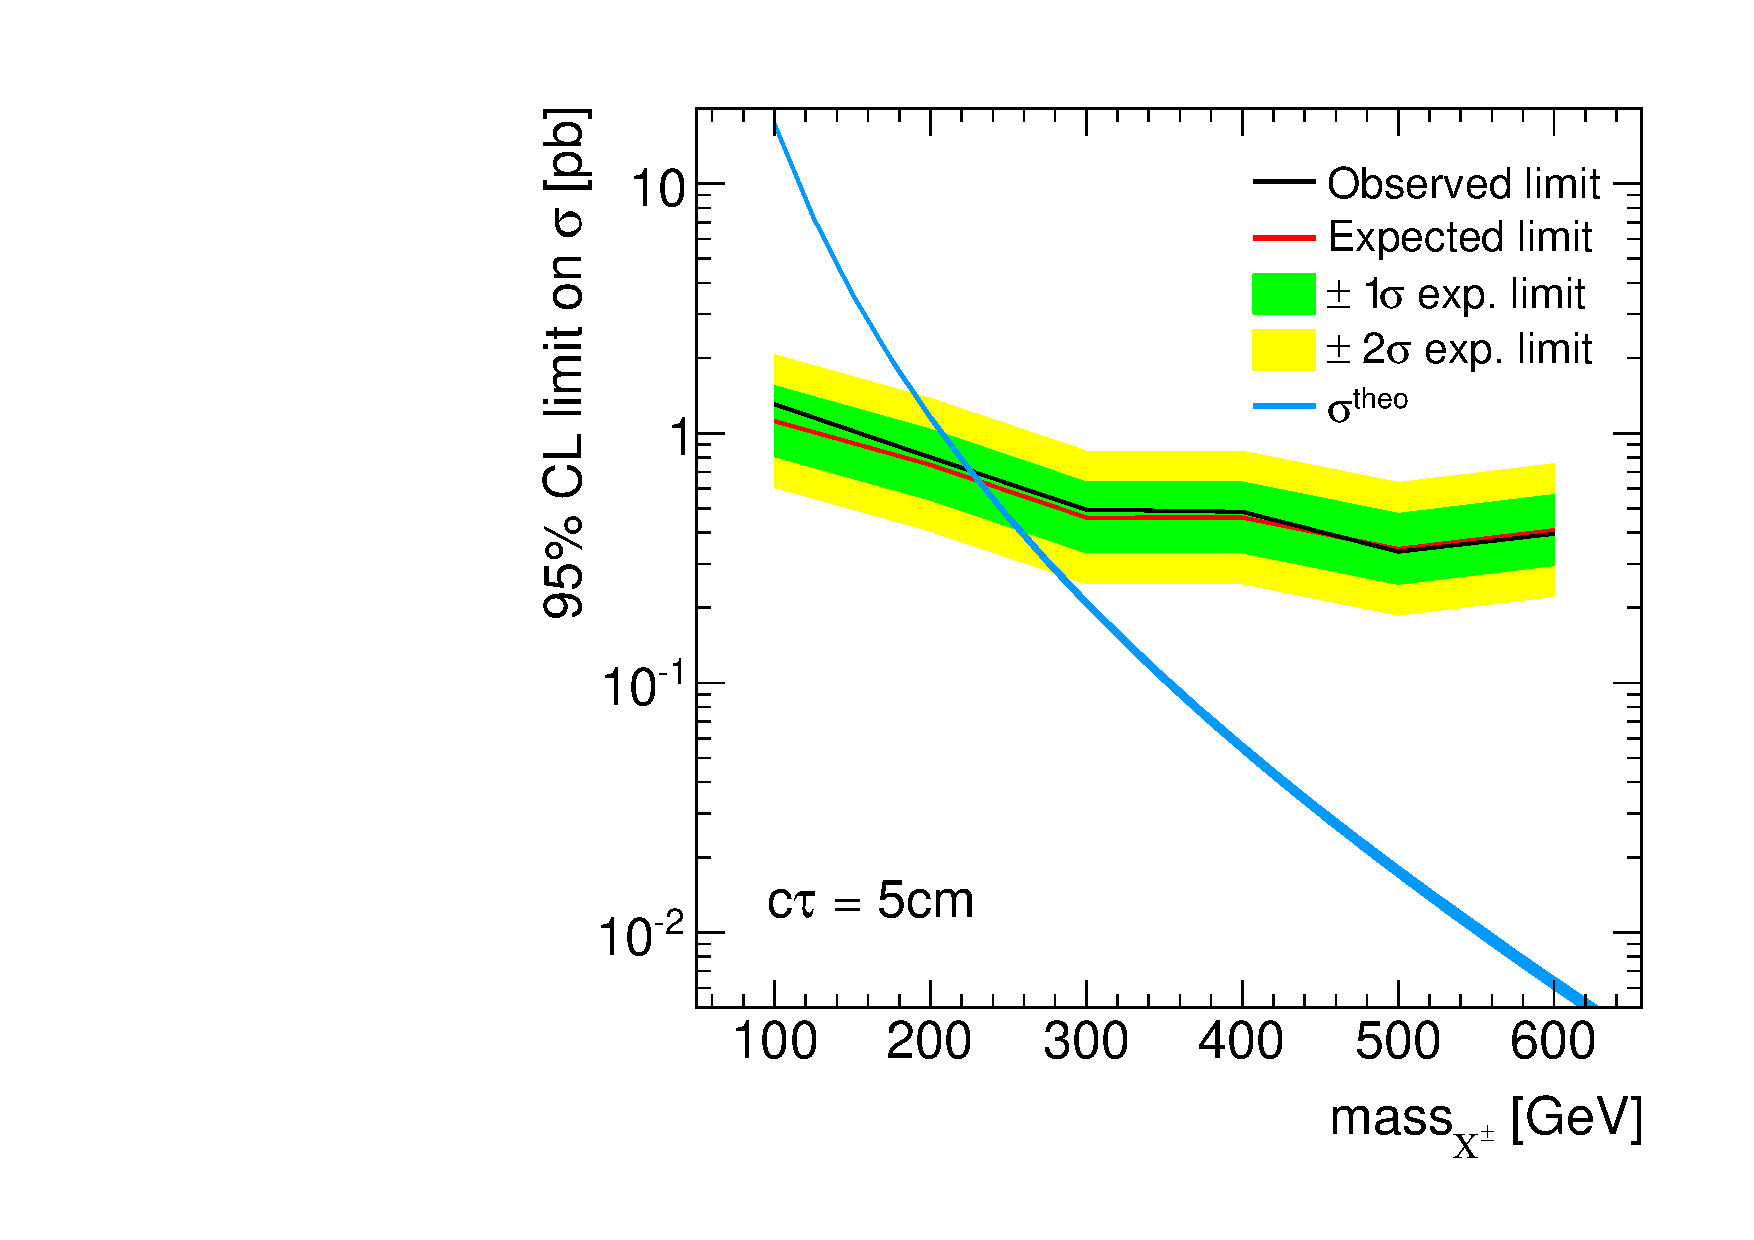
\includegraphics[width=0.49\textwidth]{figures/analysis/Interpretation/ExclusionLimits/LimitPlot_ctau5cm.pdf} 
    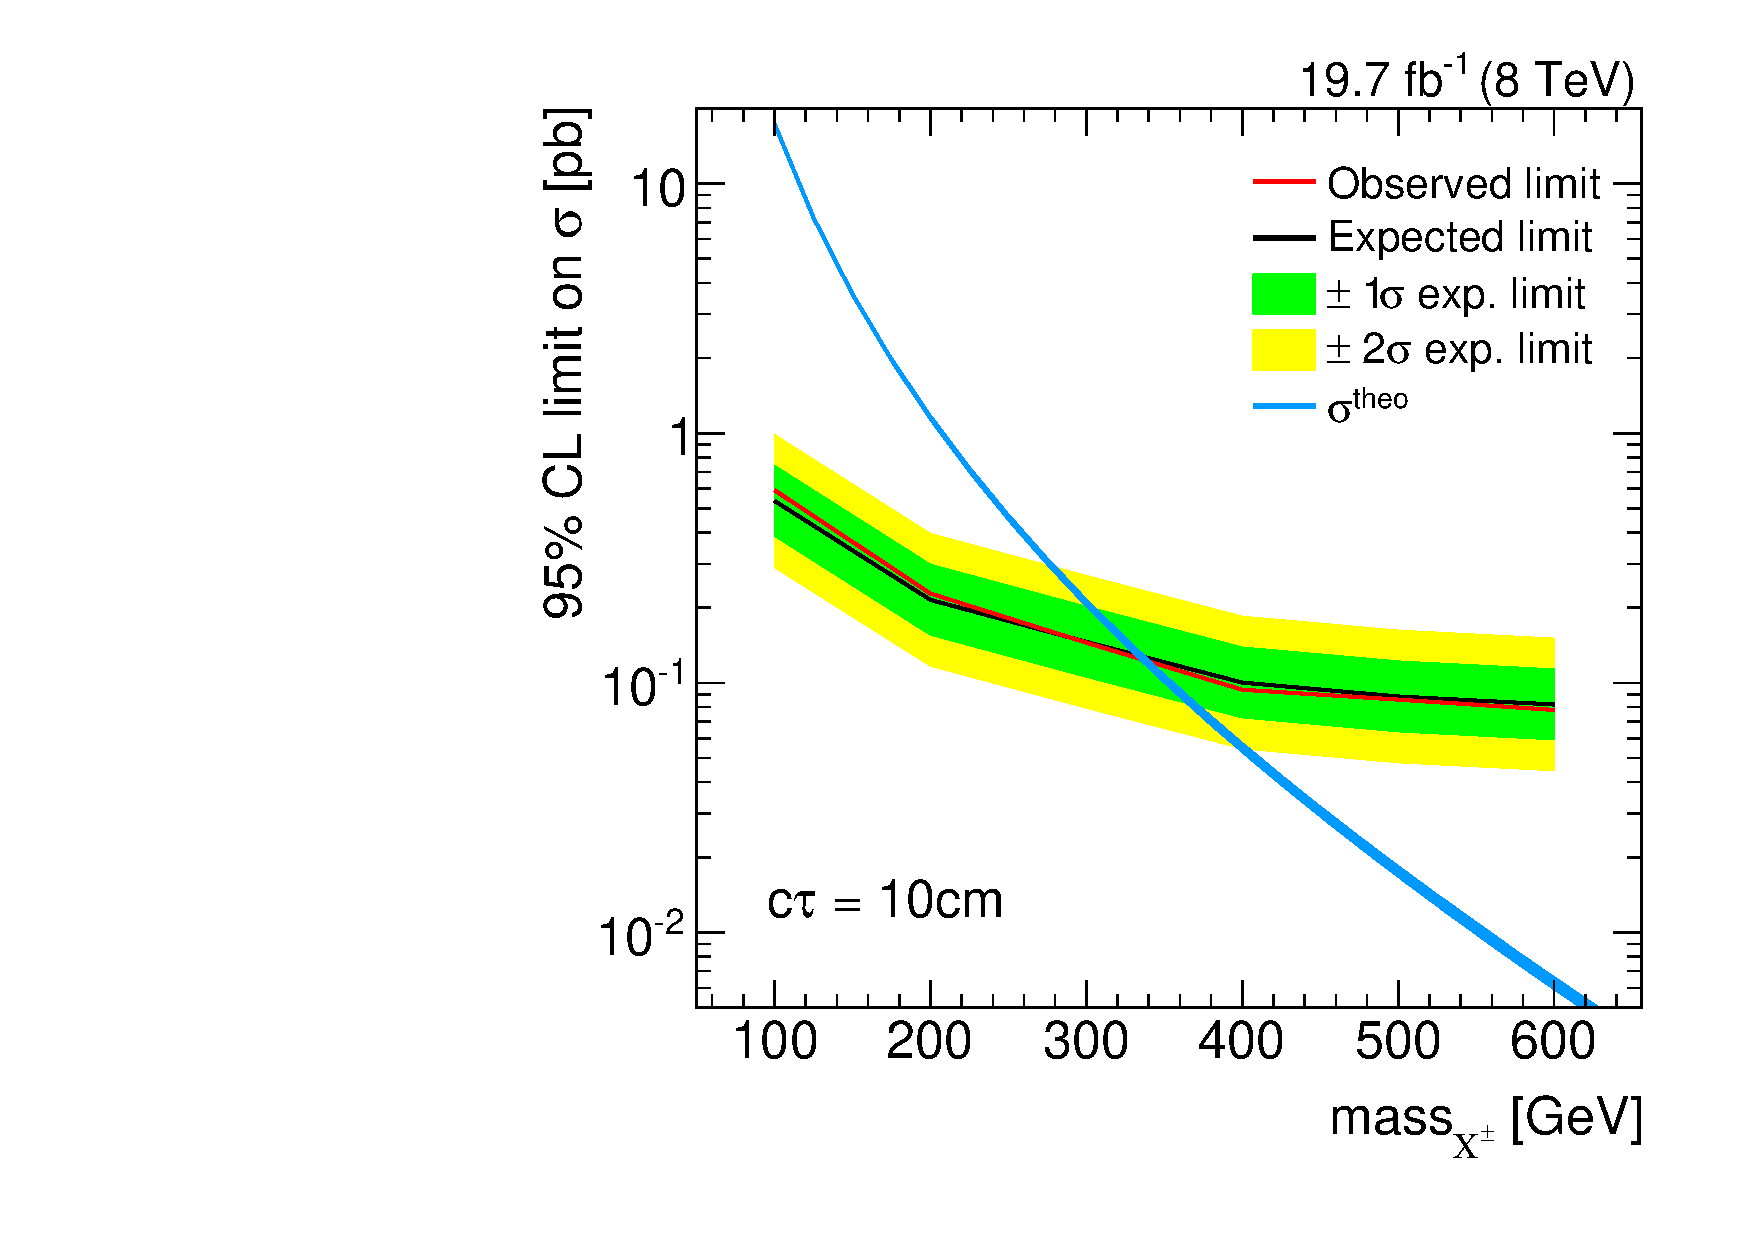
\includegraphics[width=0.49\textwidth]{figures/analysis/Interpretation/ExclusionLimits/LimitPlot_ctau10cm.pdf} \\
    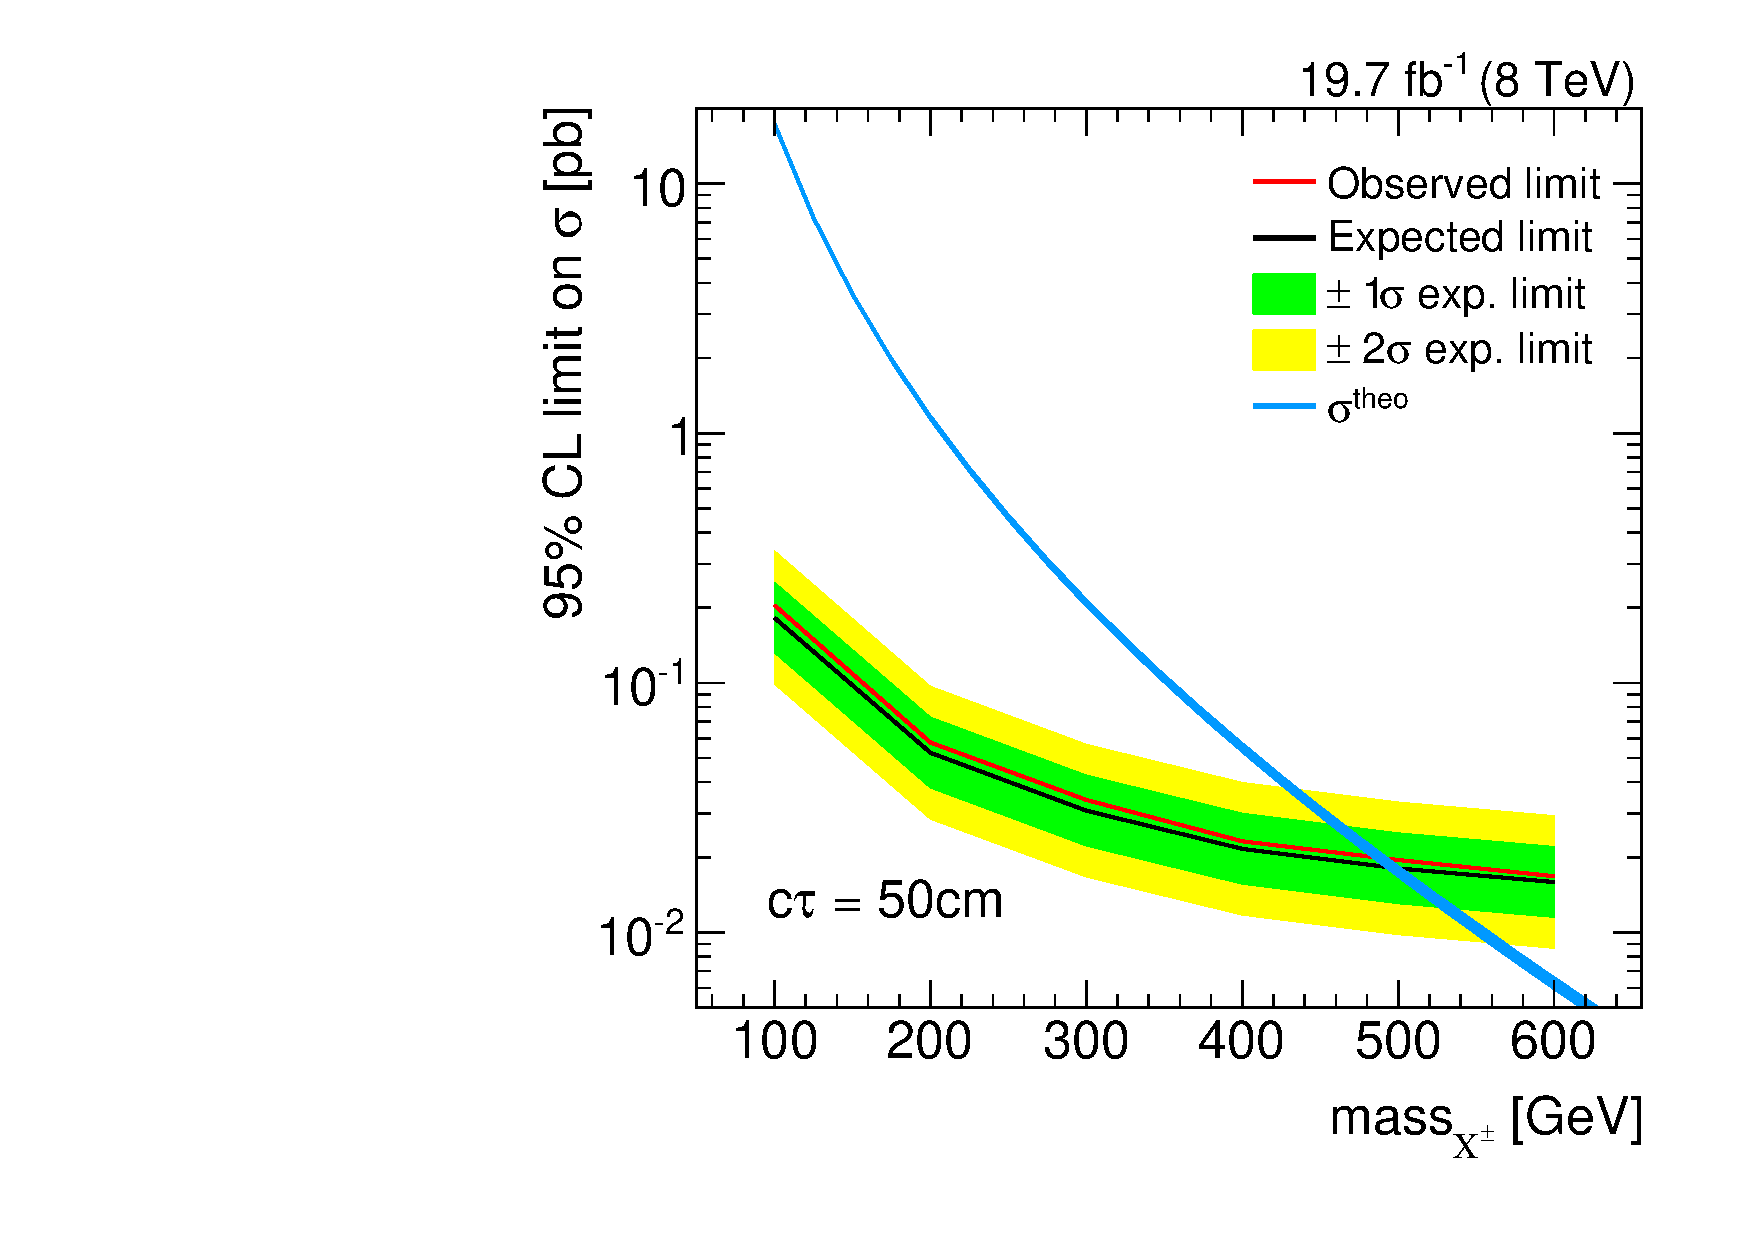
\includegraphics[width=0.49\textwidth]{figures/analysis/Interpretation/ExclusionLimits/LimitPlot_ctau50cm.pdf} 
    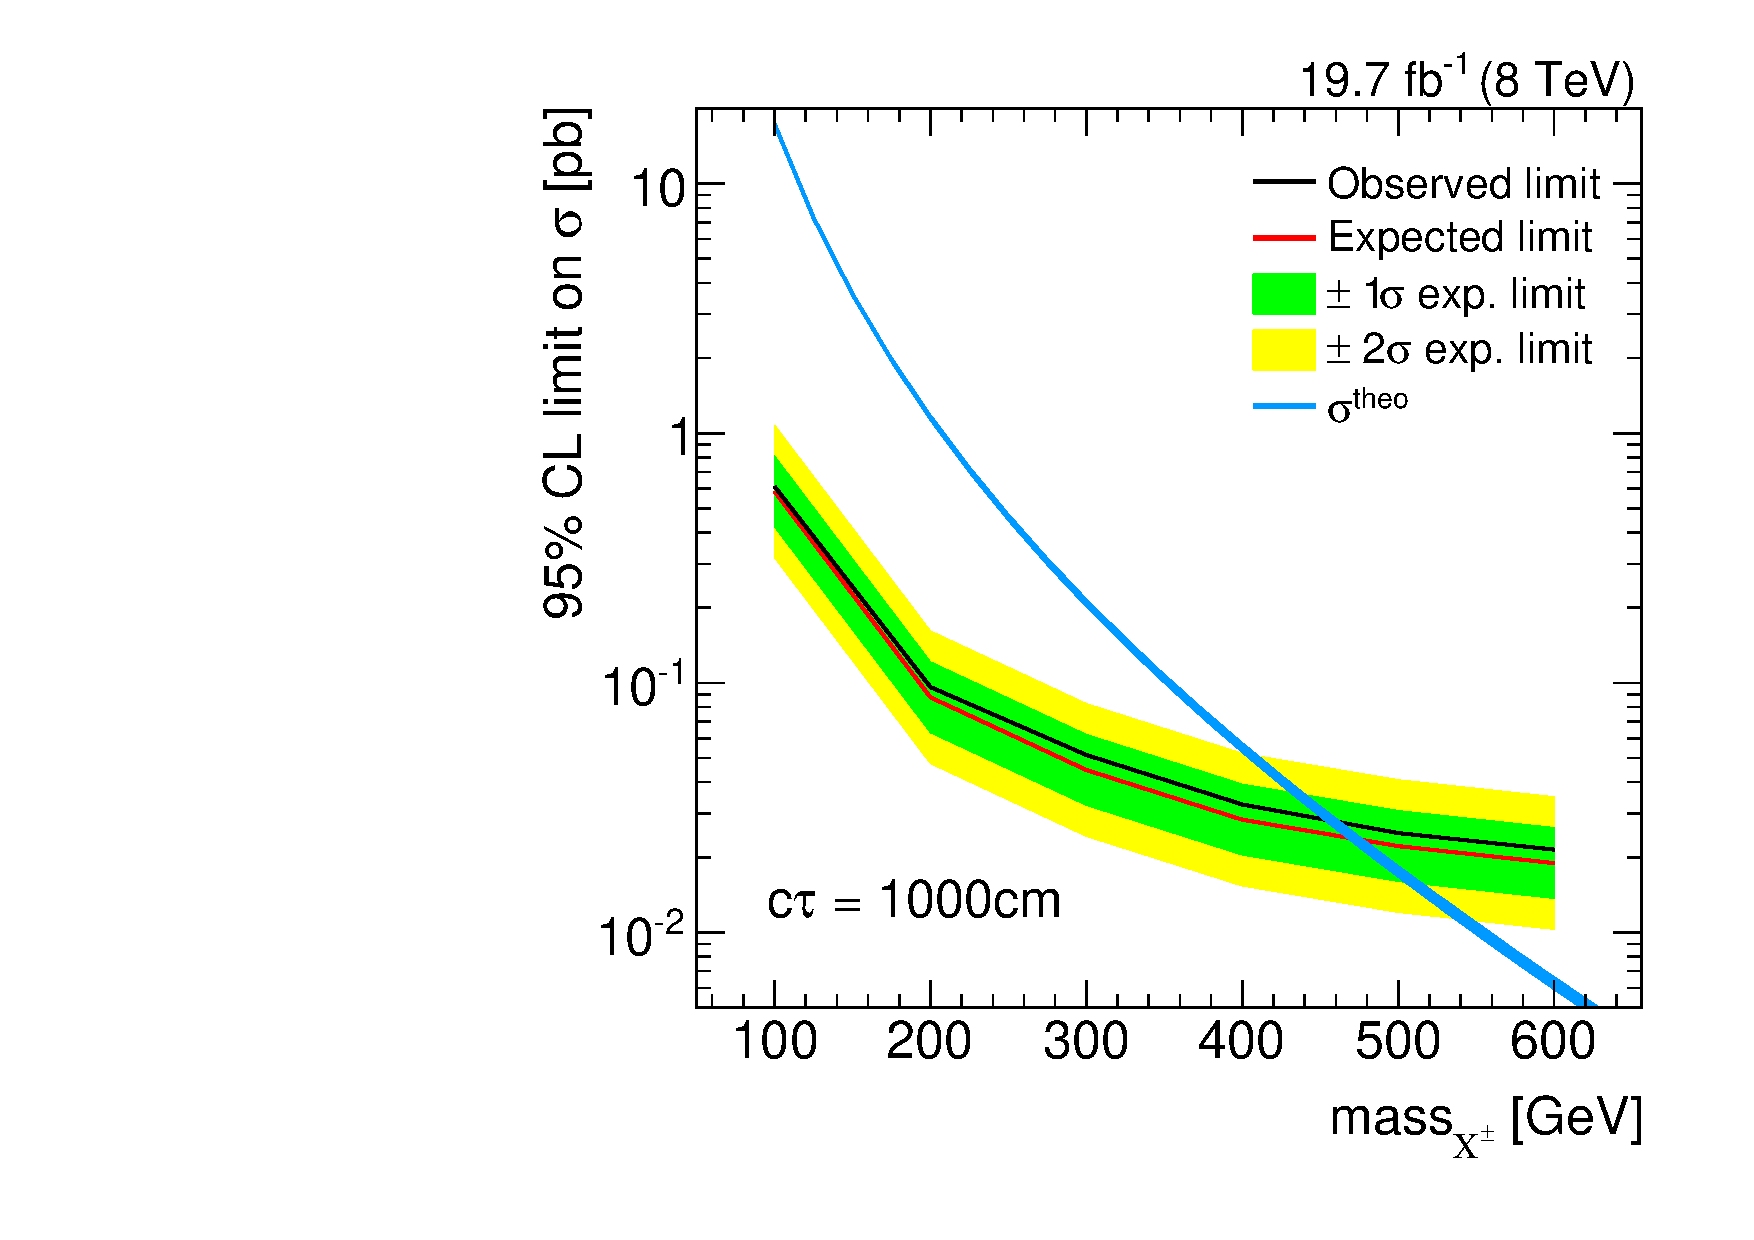
\includegraphics[width=0.49\textwidth]{figures/analysis/Interpretation/ExclusionLimits/LimitPlot_ctau1000cm.pdf} 
  \end{tabular}
  \caption{Four different \CLs exclusion limits for charginos with mean lifetimes of 5\cm (top left), 10\cm (top right), 50\cm (bottom left), 1000\cm (bottom right).
           The red line depicts the expected 95\% confidence level (CL) upper cross-section limit with the 1-$\sigma$ (green band) and 2-$\sigma$ (yellow band) intervals.
           The black line is the observed limit.
           The signal cross section is depicted as a blue line. 
           SUSY models can be excluded at 95\% CL if the signal cross section is at least as large as the 95\% CL observed upper limit on the cross section.}
  \label{fig:1dLimits}
\end{figure} 
The upper 95\% confidence level (CL) limit on the signal cross section is strongest for lifetimes between $10-100\cm$.
For lower lifetimes a sizable fraction of the charginos already decay before reaching the tracker.
For longer lifetimes, the cross section upper limit gets weaker again because the charginos start to be reconstructed as muons and do not pass the muon veto.
Also, the \ecalo requirement rejects these charginos with higher efficiency.

Due to the falling spectrum of the chargino production cross section, charginos with lower masses are more effectively excluded than charginos with higher masses.
A 2-dimensional exclusion limit in the chargino lifetime-mass parameter space is shown in Fig.~\ref{fig:2dLimit}.
\begin{figure}[!t]
  \centering 
  \begin{tabular}{c}
    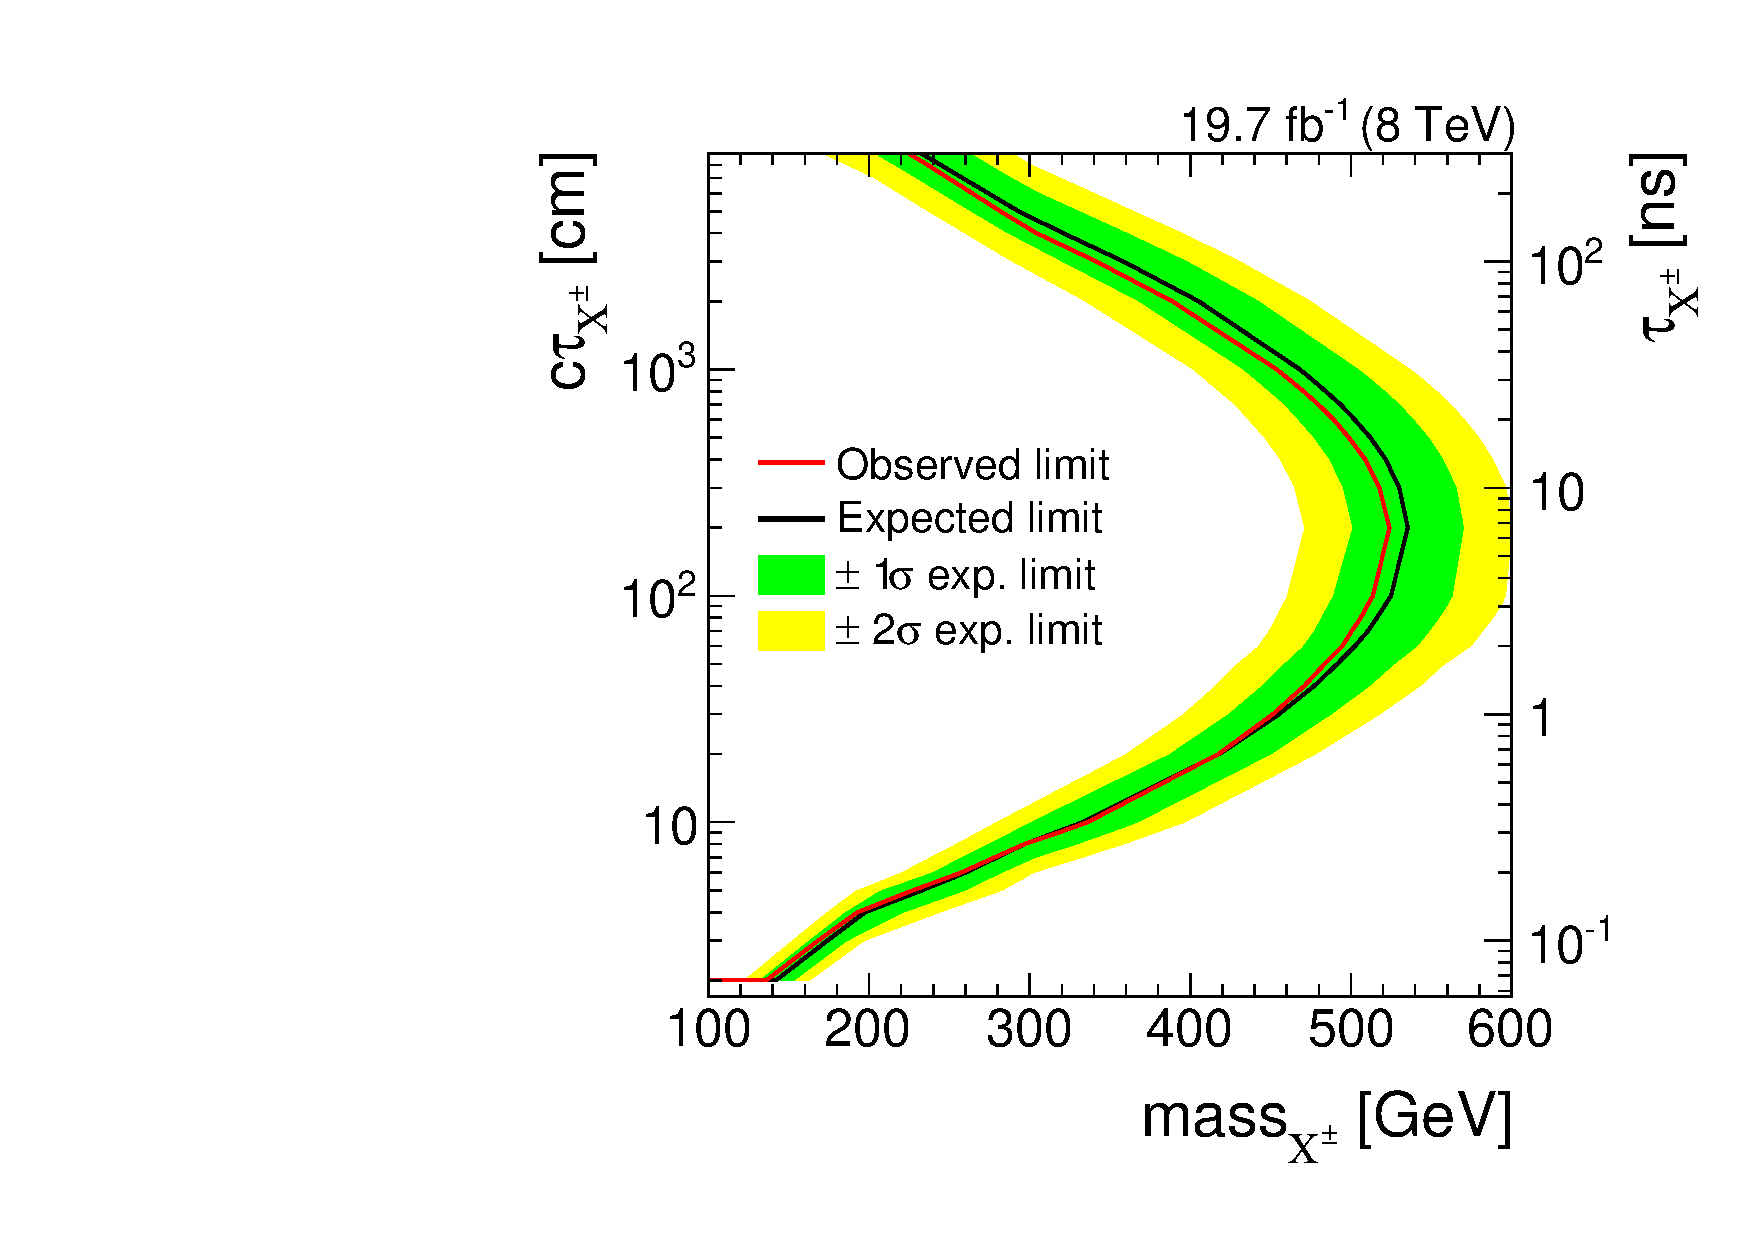
\includegraphics[width=0.79\textwidth]{figures/analysis/Interpretation/ExclusionLimits/LimitPlot_2d_log_cm.pdf} 
  \end{tabular}
  \caption{Excluded regions in the mass versus lifetime space.
           All excluded models are located left of the contour line.
            The red line depicts the expected 95\% CL upper cross-section limit with the 1-$\sigma$ (green band) and 2-$\sigma$ (yellow band) intervals.
           The black line is the observed limit.}
  \label{fig:2dLimit}
\end{figure} 

Charginos with masses of 100\gev can be excluded down to a lifetime of $\ctau=2\cm$.
Charginos with a higher mass of 500\gev are excluded for lifetimes between $\ctau=70-500\cm$.

Since the lifetime of a wino-like chargino is determined by the mass splitting between $m_{\chipm}$ and $m_{\chiO}$, 
it is possible to express the lifetime of the chargino as a mass gap $\Delta m_{\chipm\chiO}$ between the chargino and the lightest neutralino.
The correspondence between lifetime and mass gap is taken from~\cite{bib:MassSplitting_Drees}, where the decay width of $\chipm \rightarrow \chiO\, \pi^{\pm}$ is expressed in terms of chargino, neutralino, and pion mass.
Thus, the mass gaps that are considered are bounded by the pion mass of $\sim140\mev$.
The corresponding 2d exclusion limit can be found in Fig.~\ref{fig:DeltaMLimit2d}.
\begin{figure}[!t]
  \centering 
  \begin{tabular}{c}
    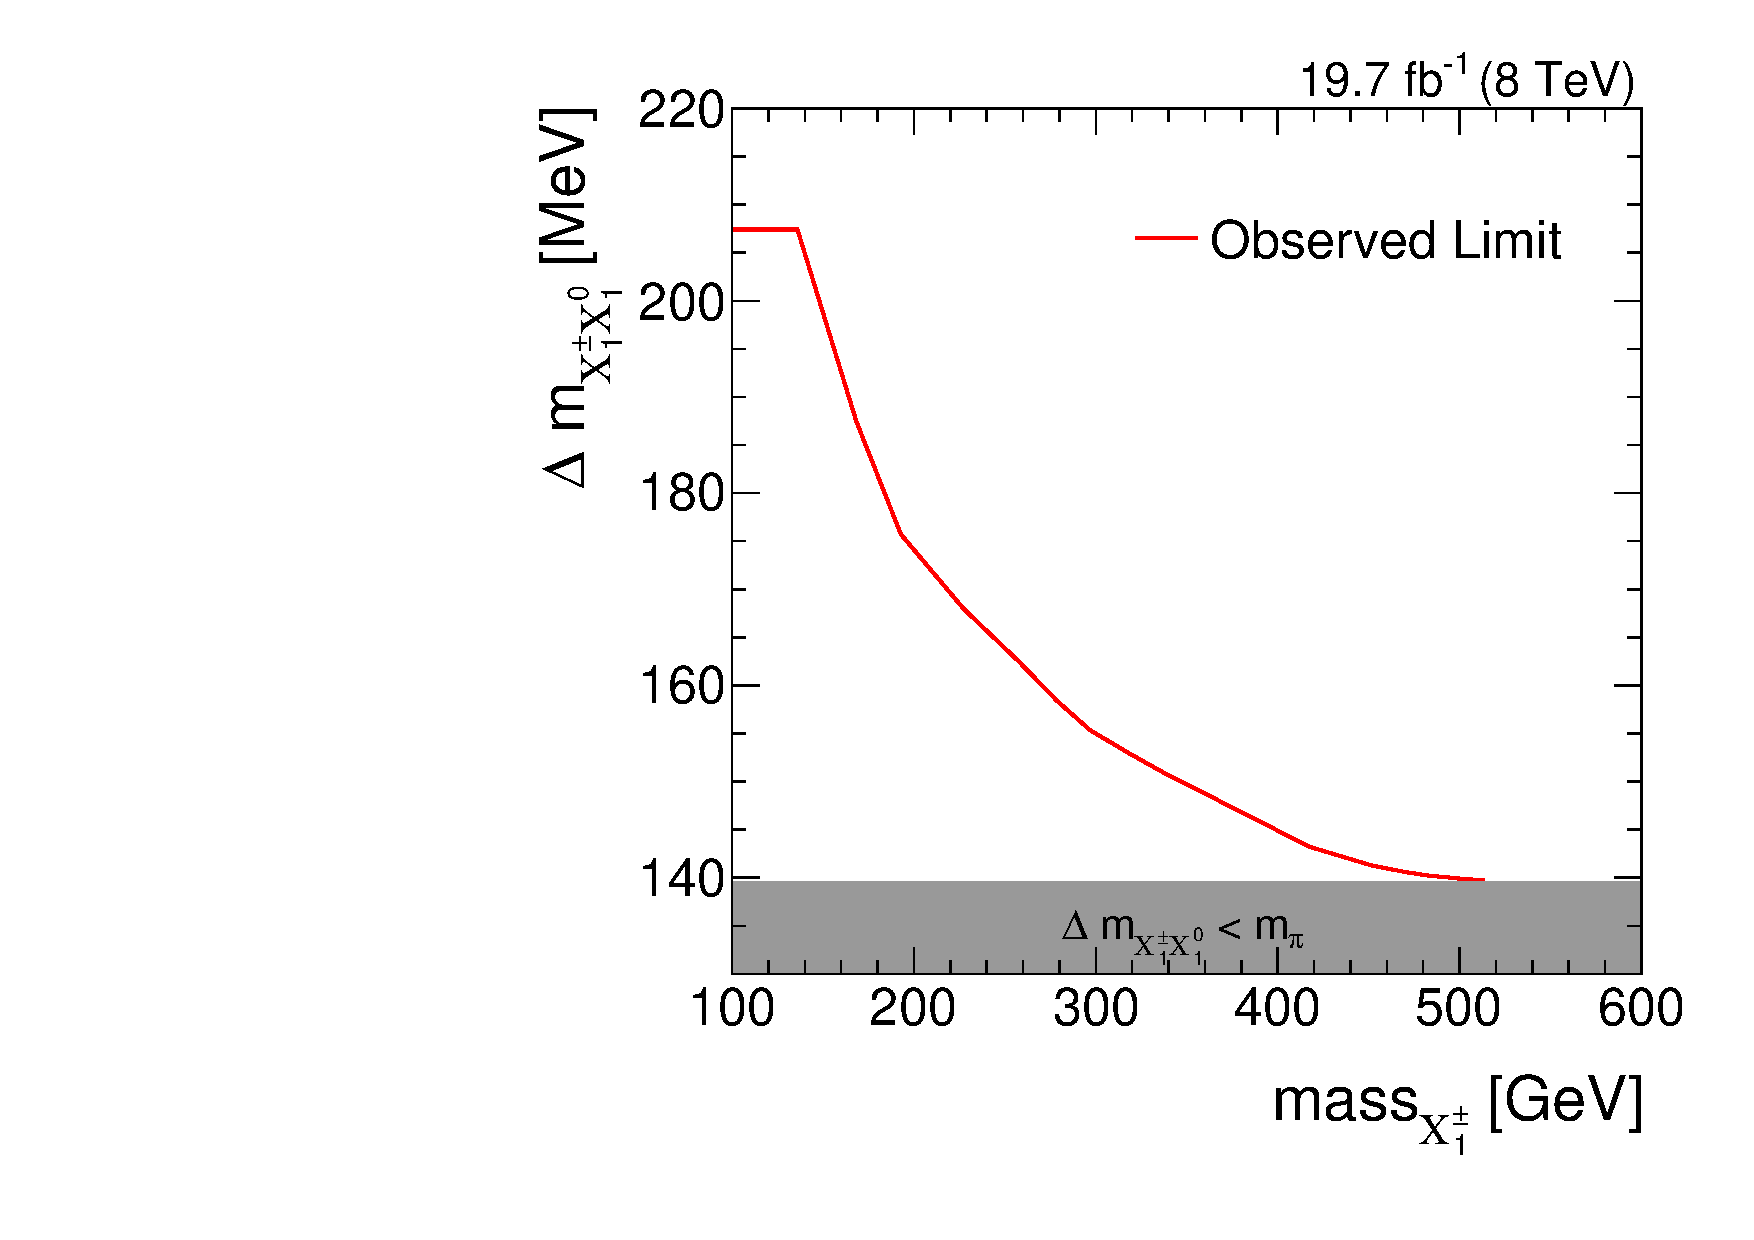
\includegraphics[width=0.55\textwidth]{figures/analysis/Interpretation/MassSplittingLimitPlot.pdf} 
  \end{tabular}
  \caption{Excluded parameter region at 95\% CL for wino-like charginos and neutralinos depending on the chargino mass and the mass splitting between \chipm and \chiO, $\Delta m_{\chipm\chiO}$.
          All SUSY models between the red line and the grey area are excluded.}
  \label{fig:DeltaMLimit2d}
\end{figure} 
It can be seen that this search is sensitive to mass splittings between $\sim 140\mev-210\mev$.\\

The presented exclusion limits confirm the exclusion from the search for disappearing tracks~\cite{bib:CMS:DT_8TeV} with slight improvements in the low lifetime region.
The comparison of the two searches is shown in Fig~\ref{fig:Comparison2dLimit}.

For charginos with a lifetime of $\tau=0.07\ns$ ($\ctau=2.1\cm$), the observed limit of this search improves the limits derived in~\cite{bib:CMS:DT_8TeV} by $\sim35\gev$ in chargino mass, for a lifetime of $\tau=0.4\ns$ ($\ctau=12.0\cm$) by $\sim25\gev$. 
For SUSY models with long chargino lifetimes the here presented search shows a higher exclusion power.
The weaker exclusion for long lifetimes in~\cite{bib:CMS:DT_8TeV} is caused by the additional selection cut on the number of missing outer hits, $\nlostouter\geq3$.

The confirmation of the excluded parameter space in~\cite{bib:CMS:DT_8TeV} is especially interesting since the signal regions of the two searches are little correlated.
The correlation between simulated signal events, that pass the selection from~\cite{bib:CMS:DT_8TeV}, $N_A$, and the selection used in this analysis, $N_B$, can be estimated by the event overlap $\rho_{\text{corr}}$
\begin{equation*}
\rho_{\text{corr}} = \frac{N_{A\cap B}}{N_{A \cup B}} = \frac{N_{A\cap B}}{N_A + N_B - N_{A \cap B}}.
\end{equation*}
In order to avoid an over- or underestimation of the event overlap, only the most sensitive signal region from this search is included in $N_B$.
The degree of correlation is depicted in Fig.~\ref{fig:AnalysisOverlap} which shows the event overlap for signal models with chargino masses between $100-600\gev$ and lifetimes between $5\cm-1000\cm$.
\begin{figure}[!t]
  \centering 
  \begin{tabular}{c}
    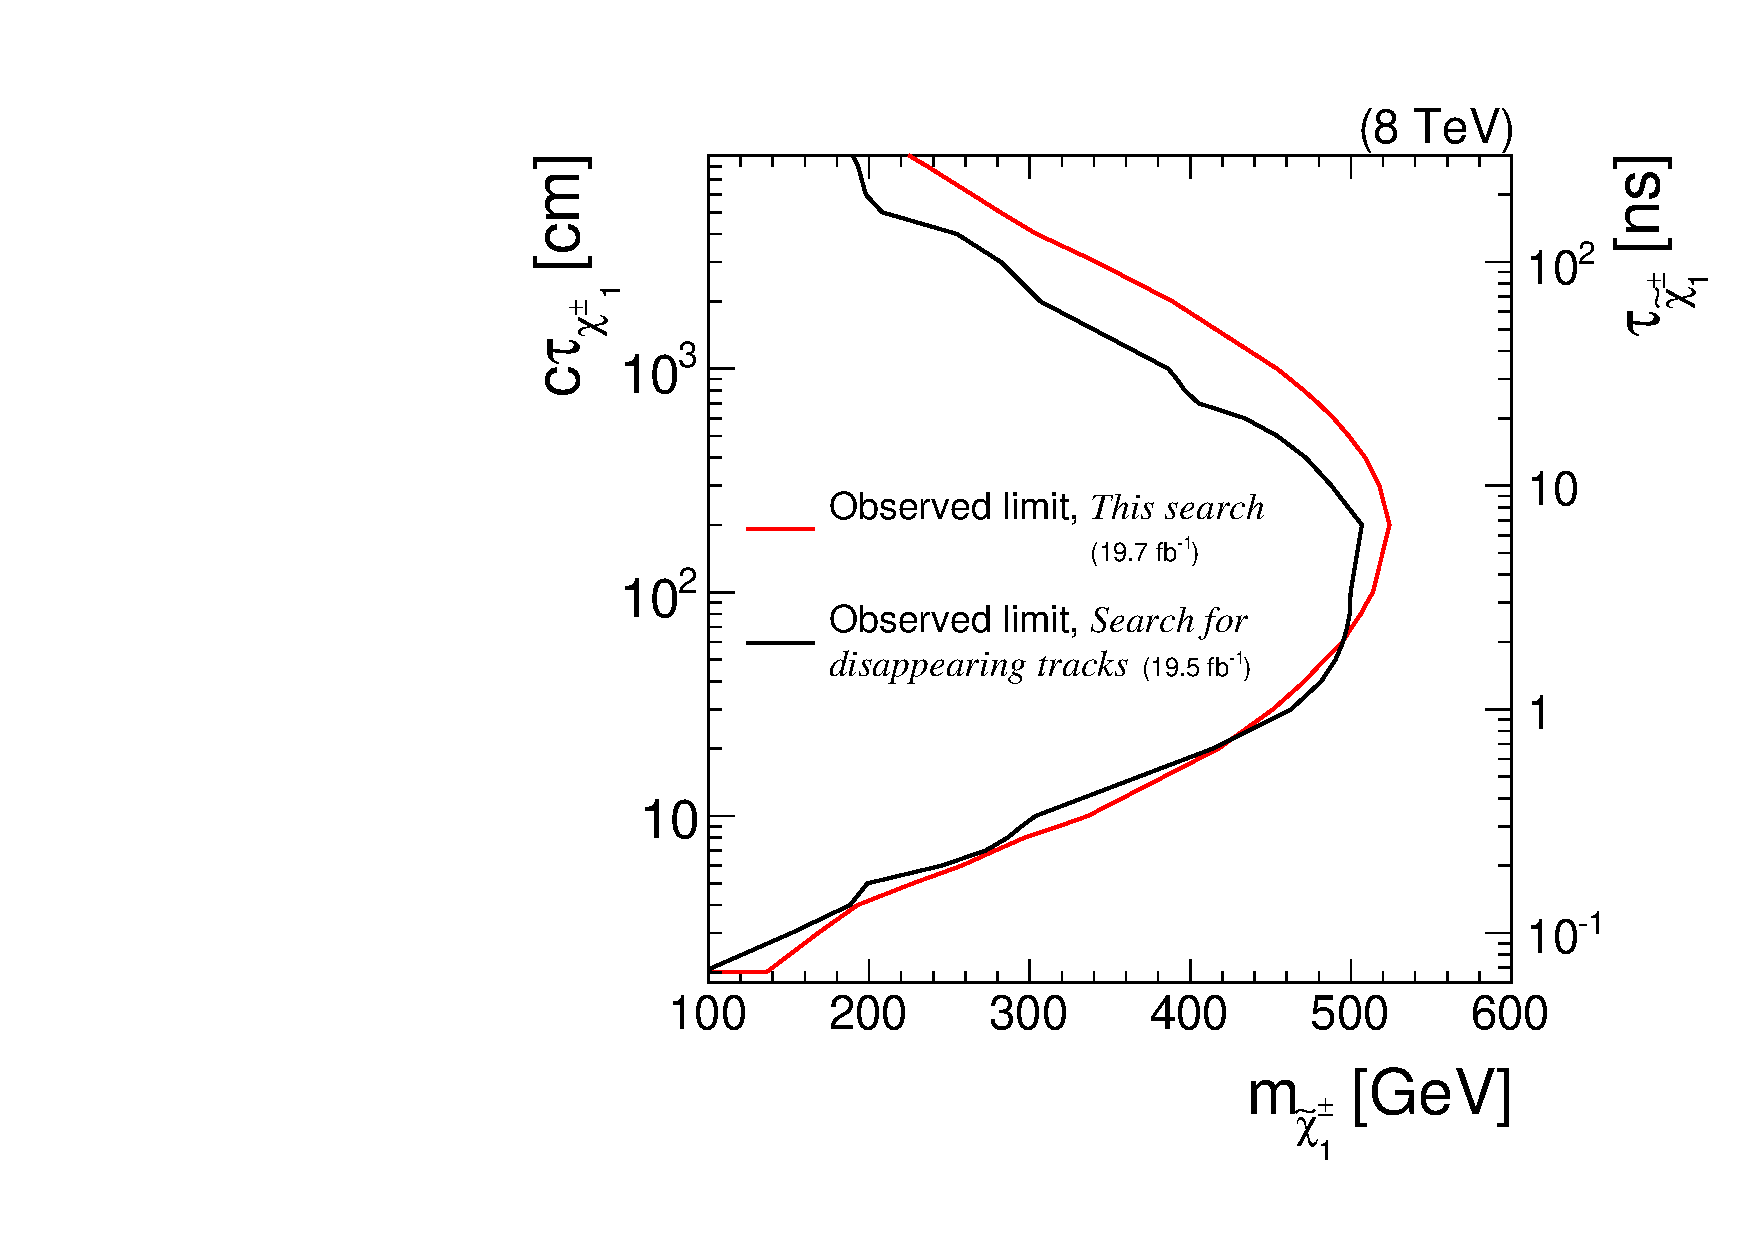
\includegraphics[width=0.49\textwidth]{figures/analysis/Interpretation/Comparison2dLimits_largerRange.pdf}  
    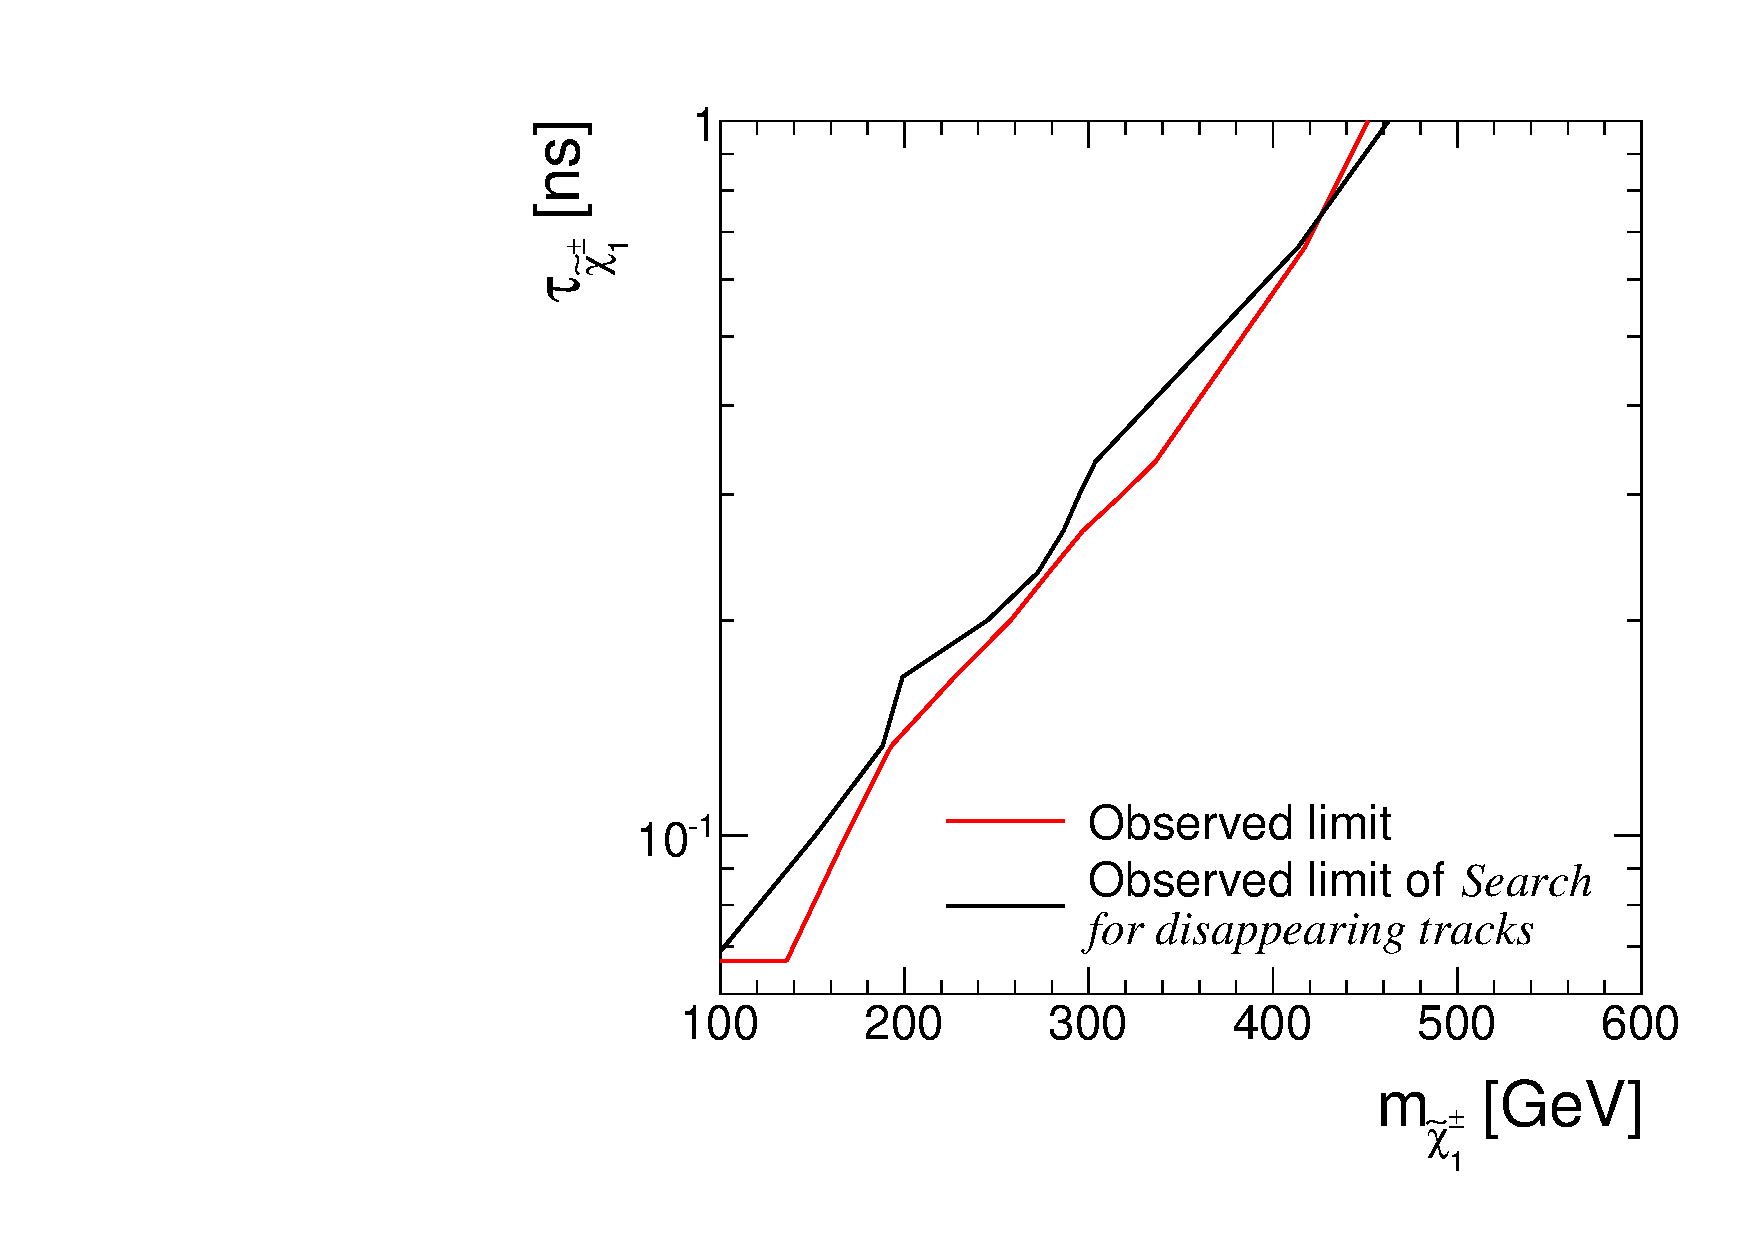
\includegraphics[width=0.49\textwidth]{figures/analysis/Interpretation/Comparison2dLimits.pdf} 
  \end{tabular}
  \caption{Comparison of the excluded regions in the mass versus lifetime space in this analysis (red line) and the search for disappearing tracks~\cite{bib:CMS:DT_8TeV} (black line). 
           The right figure is a zoom on the low lifetime region. All SUSY models left of the lines are excluded.}
  \label{fig:Comparison2dLimit}
\end{figure} 
\begin{figure}[!b]
\vspace{20pt}
  \centering 
  \begin{tabular}{c}
    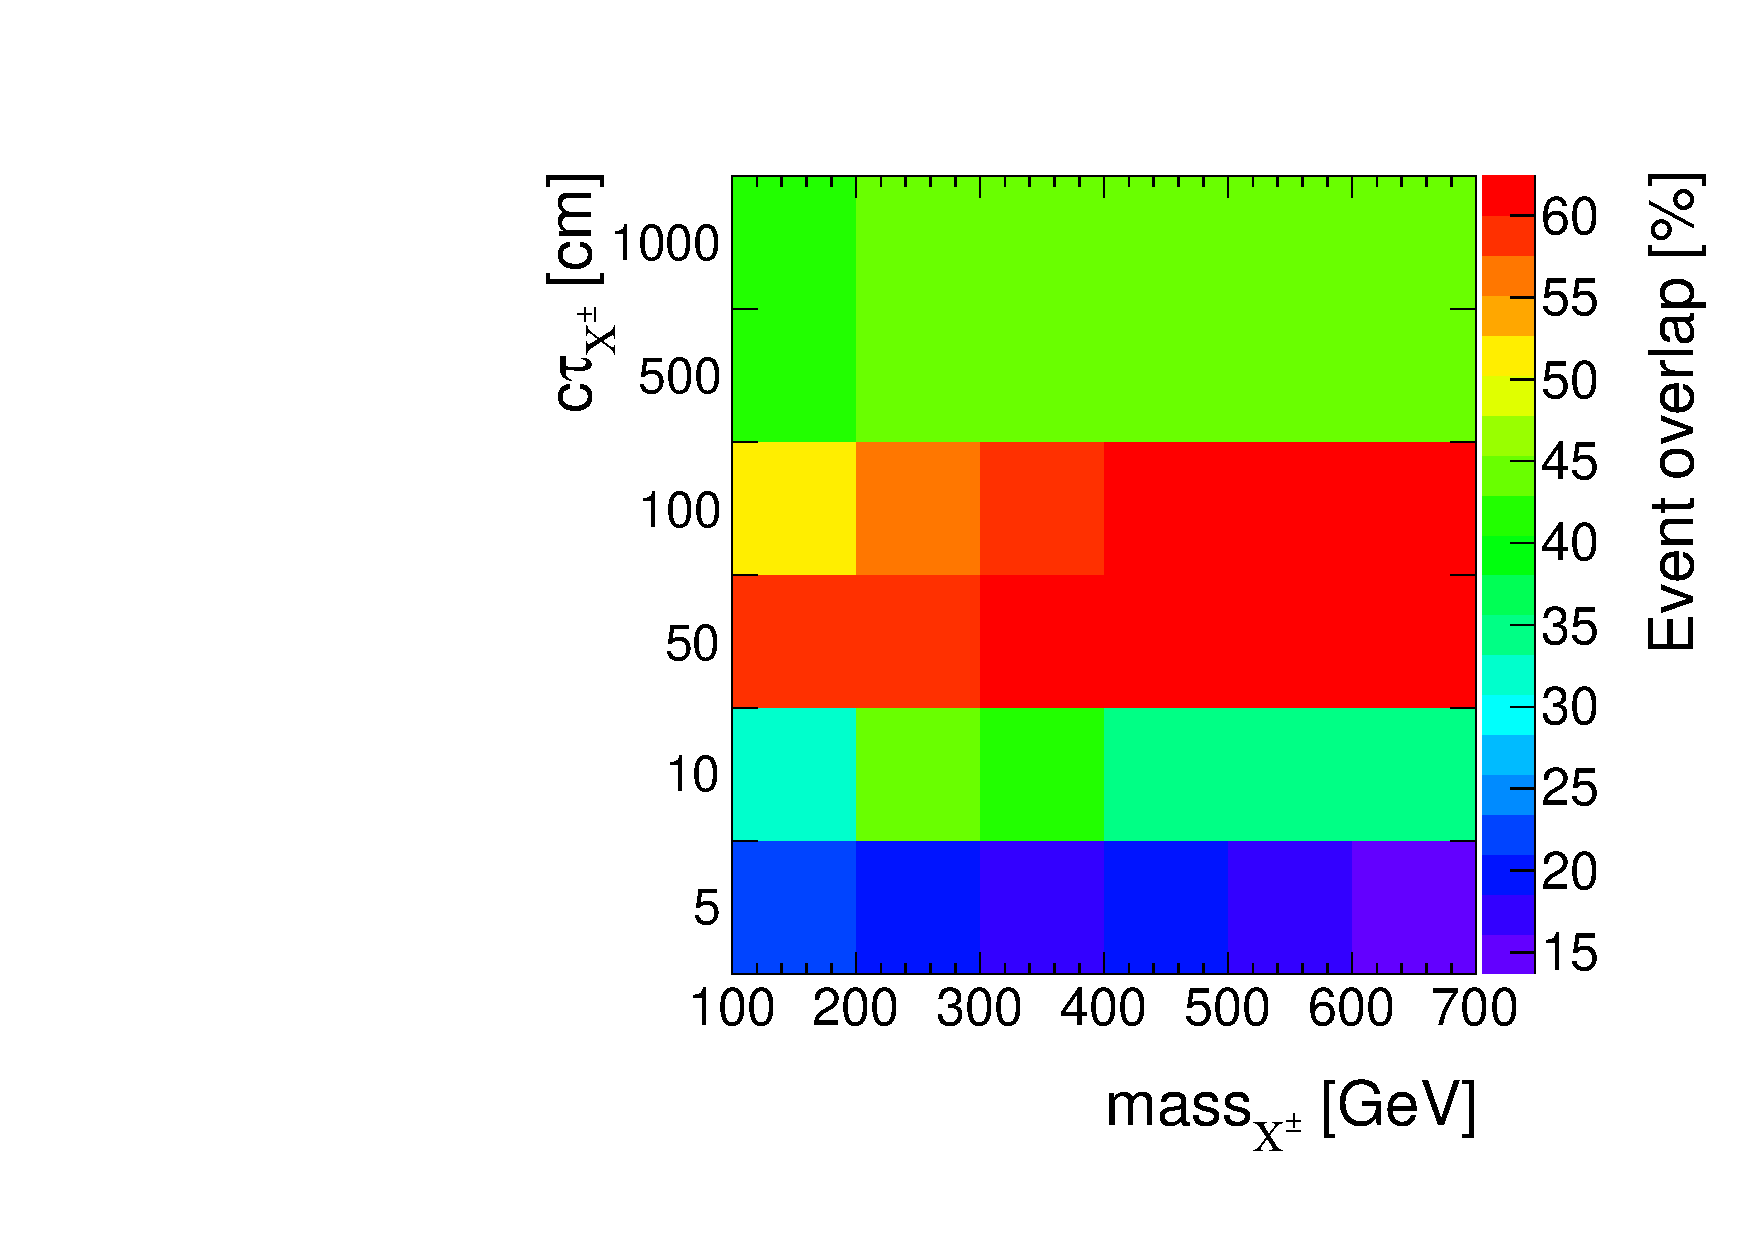
\includegraphics[width=0.49\textwidth]{figures/analysis/Interpretation/AnalysisOverlap.pdf}  
  \end{tabular}
  \caption{The event overlap between simulated signal events, that pass the selection from~\cite{bib:CMS:DT_8TeV} and the selection used in this analysis for different signal models.
          The correlation is determined using only the signal region with the highest sensitivity of this analysis.}
  \label{fig:AnalysisOverlap}
\end{figure} 
It can be seen that the event overlap for intermediate lifetimes of around 100\cm is around 60\% and decreases for shorter lifetimes to small overlaps of around $15-20\%$.
Additionally, the two events that were observed in data by~\cite{bib:CMS:DT_8TeV} in their signal region are not contained in any of the signal regions in the here presented analysis.
Thus, this analysis constitutes an independent confirmation of the exclusion limits derived in~\cite{bib:CMS:DT_8TeV}.

% with an almost independent set of simulated signal events for low lifetimes.
%It should also be noted that the two events observed in data in the signal region of~\cite{bib:CMS:DT_8TeV}, are not contained in any of the signal regions in the here presented analysis.
%One event is rejected by the tighter calorimeter isolation requirement of $\ecalo<5\gev$ (cf.~\cite{bib:CMS:DT_8TeV} required $\ecalo<10\gev$), and the other event is rejected by the stronger QCD suppression requirements.
%Thus, also the observed data shows no event overlap between this search and the search from~\cite{bib:CMS:DT_8TeV}.



%%%%%%%%%%%%%%%%%%%%%%%%%%%%%%%%%%%%%%%%%%%%%%%%%%%%%%%%%%%%%%%%%%%%%%%%%%%%%%%%%%%%%%%%%%%%%%%%%%%%%%%%%%%%%%%%%%%%%%%%%%%%%%%%%%%%%%%%%%%%%%%%%%%%%%%%%%%%%%%%%%%%%%%
%%%%%%%%%%%%%%%%%%%%%%%%%%%%%%%%%%%%%%%%%%%%%%%%%%%%%%%%%%%%%%%%%%%%%%%%%%%%%%%%%%%%%%%%%%%%%%%%%%%%%%%%%%%%%%%%%%%%%%%%%%%%%%%%%%%%%%%%%%%%%%%%%%%%%%%%%%%%%%%%%%%%%%%
%%%%%%%%%%%%%%%%%%%%%%%%%%%%%%%%%%%%%%%%%%%%%%%%%%%%%%%%%%%%%%%%%%%%%%%%%%%%%%%%%%%%%%%%%%%%%%%%%%%%%%%%%%%%%%%%%%%%%%%%%%%%%%%%%%%%%%%%%%%%%%%%%%%%%%%%%%%%%%%%%%%%%%%
\FloatBarrier
\chapter{Discussion and conclusion}
\label{sec:Discussion}

The here presented search for highly ionising, short tracks is motivated by supersymmetric models with almost mass-degenerate wino-like charginos \chipm and neutralinos \chiO.
Such scenarios are well motivated by astrophysical observations that suggest the existence of large amounts of dark matter.
It is possible to explain the relic density with wino-like neutralinos if they are non-thermally produced via the decay of long-lived particles, such as a wino-like chargino~\cite{bib:Moroi:DarkMatter_2013}.\\

The presented analysis is designed to increase the search sensitivity on SUSY models with low chargino lifetimes.
It extends the search for disappearing tracks~\cite{bib:CMS:DT_8TeV} by the inclusion of the variable \dedx.
In order to increase the search sensitivity with respect to short lifetimes, energy information from the pixel silicon tracker is taken into account.
For this purpose, a dedicated pixel energy calibration was carried out within this thesis to ensure stable energy measurements over time and across pixel modules.
This is thus the first analysis at CMS that makes use of energy information from the pixel tracker.
By adding pixel energy information the discrimination power of \dedx is significantly increased.

Overall, \dedx inclusion allows for loosening the requirement on the number of hits in the tracker with respect to~\cite{bib:CMS:DT_8TeV} that leads to a strong suppression of signal events for low chargino lifetimes. 
The Asymmetric Smirnov discriminator, \ias, which is used for \dedx discrimination in this analysis, shows good separation power and can lead to sensitivity increases up to 400\% (cf. Fig.~\ref{fig:optimisation}).\\


The Standard Model background is mainly estimated with data-based techniques.
The main background to this search is arising from fake tracks, \ie tracks that are reconstructed out of several particles' trajectories.
Fake tracks are typically short and can have large values of \ias, thus showing a very signal-like signature in the detector.
The uncertainty on the fake background is dominated by systematic uncertainties originating from low statistical precision in the simulated datasets.
Simulating more events could therefore significantly improve the search sensitivity.
This strategy is however technically challenging, since storage capacity limits were already reached within the current analysis.
Still, reducing the uncertainty will be one of the main tasks in order to increase the search sensitivity.

Even though this search already features low background, a further background suppression is desirable.
However, the impact on the search sensitivity will be limited because of the high relative Poisson error on low background predictions.
For instance, a reduction of the number of background events by 75\% from 4 to 1 event reduces the signal yield required for a 5$\sigma$-discovery by around 30\%, whereas a 75\% reduction of expected background events from 400 to 100 reduces the required signal yield by 70\%.

In the current analysis, the background is estimated at $19-24$ events in the low \ias signal regions and $2.5-2.6$ events in the high \ias regions.
This background estimate is confronted with collision data recorded during the year 2012 at the CMS experiment at a centre-of-mass energy of 8\tev.
%Collision data recorded during the year 2012 at the CMS experiment at a centre-of-mass energy of 8\tev was analysed with respect to SUSY scenarios with almost mass-degenerate charginos and neutralinos.
No evidence for physics beyond the Standard Model is found. % since the observations are compatible with SM expectations within $1\sigma$.
Thus, the absence of any deviation from the Standard Model prediction is used to constrain the supersymmetric parameter space.
Wino-like charginos are excluded down to lifetimes of $\ctau=2\cm$ for $m_{\chipm}=100\gev$.
For high mass scenarios of $m_{\chipm}=500\gev$, the excluded lifetime ranges between $\ctau=70-500\cm$.
This confirms the parameter exclusion limits of the search for disappearing tracks~\cite{bib:CMS:DT_8TeV}.
Interestingly, the signal regions of the here presented search and the search from~\cite{bib:CMS:DT_8TeV} show little overlap.
Therefore, this analysis serves as an independent cross check of~\cite{bib:CMS:DT_8TeV}.
Improvements of the exclusion of SUSY models with respect to existing searches of around $10-40\gev$ in chargino mass are achieved in the low lifetime region.\\

Still, SUSY models with higher mass and low lifetimes could not be fully excluded by any search at the LHC.
Therefore, it will stay interesting to further search for these phenomenologically interesting scenarios in collisions at a centre-of-mass energy of 13\tev.
In this context, the here presented approach of combining a selection of short tracks with \dedx information is especially promising.
The expected cross section for SUSY models with higher chargino masses of around 500\gev will increase by a factor of two at $\sqrt{s}= 13\tev$.
Since \dedx is much more discriminating for high masses, the sensitivity impact is expected to be even more pronounced for 13\tev data.

%Up to now, no evidence for Supersymmetry at the LHC could be found.
%Still, such an explanatory powerful and aesthetically convincing theory will not be given up without a certain confidence that it is not realised in nature.
%That makes especially exotic searches very interesting and it will remain requisite to look also in the little exotic corners of Supersymmetry in the future.

